% ******************************* PhD Thesis Template **************************
% Please have a look at the README.md file for info on how to use the template

\documentclass[a4paper,10pt,times,numbered,print,index]{Classes/PhDThesisPSnPDF}

% ******************************************************************************
% ******************************* Class Options ********************************
% *********************** See README for more details **************************
% ******************************************************************************

% `a4paper'(The University of Cambridge PhD thesis guidelines recommends a page
% size a4 - default option) or `a5paper': A5 Paper size is also allowed as per
% the Cambridge University Engineering Deparment guidelines for PhD thesis
%
% `11pt' or `12pt'(default): Font Size 10pt is NOT recommended by the University
% guidelines
%
% `oneside' or `twoside'(default): Printing double side (twoside) or single
% side.
%
% `print': Use `print' for print version with appropriate margins and page
% layout. Leaving the options field blank will activate Online version.
%
% `index': For index at the end of the thesis
%
% `draftclassic': For draft mode without loading any images (same as draft in book)
%
% `draft': Special draft mode with line numbers, images, and water mark with
% timestamp and custom text. Position of the text can also be modified.
%
% `abstract': To generate only the title page and abstract page with
% dissertation title and name, to submit to the Student Registry
%
% `chapter`: This option enables only the specified chapter and it's references
%  Useful for review and corrections.
%
% ************************* Custom Page Margins ********************************
%
% `custommargin`: Use `custommargin' in options to activate custom page margins,
% which can be defined in the preamble.tex. Custom margin will override
% print/online margin setup.
%
% *********************** Choosing the Fonts in Class Options ******************
%
% `times' : Times font with math support. (The Cambridge University guidelines
% recommend using times)
%
% `fourier': Utopia Font with Fourier Math font (Font has to be installed)
%            It's a free font.
%
% `customfont': Use `customfont' option in the document class and load the
% package in the preamble.tex
%
% default or leave empty: `Latin Modern' font will be loaded.
%
% ********************** Choosing the Bibliography style ***********************
%
% `authoryear': For author-year citation eg., Krishna (2013)
%
% `numbered': (Default Option) For numbered and sorted citation e.g., [1,5,2]
%
% `custombib': Define your own bibliography style in the `preamble.tex' file.
%              `\RequirePackage[square, sort, numbers, authoryear]{natbib}'.
%              This can be also used to load biblatex instead of natbib
%              (See Preamble)
%
% **************************** Choosing the Page Style *************************
%
% `default (leave empty)': For Page Numbers in Header (Left Even, Right Odd) and
% Chapter Name in Header (Right Even) and Section Name (Left Odd). Blank Footer.
%
% `PageStyleI': Chapter Name next & Page Number on Even Side (Left Even).
% Section Name & Page Number in Header on Odd Side (Right Odd). Footer is empty.
%
% `PageStyleII': Chapter Name on Even Side (Left Even) in Header. Section Number
% and Section Name in Header on Odd Side (Right Odd). Page numbering in footer

% Uncomment to change page style
%\pagestyle{PageStyleII}

% ********************************** Preamble **********************************
% Preamble: Contains packages and user-defined commands and settings
% ******************************************************************************
% ****************************** Custom Margin *********************************

% Add `custommargin' in the document class options to use this section
% Set {innerside margin / outerside margin / topmargin / bottom margin}  and
% other page dimensions
\ifsetCustomMargin
  \RequirePackage[left=37mm,right=30mm,top=35mm,bottom=30mm]{geometry}
  \setFancyHdr % To apply fancy header after geometry package is loaded
\fi

% Add spaces between paragraphs
%\setlength{\parskip}{0.5em}
% Ragged bottom avoids extra whitespaces between paragraphs
\raggedbottom
% To remove the excess top spacing for enumeration, list and description
%\usepackage{enumitem}
%\setlist[enumerate,itemize,description]{topsep=0em}

% *****************************************************************************
% ******************* Fonts (like different typewriter fonts etc.)*************

% Add `customfont' in the document class option to use this section

\ifsetCustomFont
  % Set your custom font here and use `customfont' in options. Leave empty to
  % load computer modern font (default LaTeX font).
  %\RequirePackage{helvet}

  % For use with XeLaTeX
  %  \setmainfont[
  %    Path              = ./libertine/opentype/,
  %    Extension         = .otf,
  %    UprightFont = LinLibertine_R,
  %    BoldFont = LinLibertine_RZ, % Linux Libertine O Regular Semibold
  %    ItalicFont = LinLibertine_RI,
  %    BoldItalicFont = LinLibertine_RZI, % Linux Libertine O Regular Semibold Italic
  %  ]
  %  {libertine}
  %  % load font from system font
  %  \newfontfamily\libertinesystemfont{Linux Libertine O}
\fi

% *****************************************************************************
% **************************** Custom Packages ********************************

% ************************* Algorithms and Pseudocode **************************

%\usepackage{algpseudocode}


% ********************Captions and Hyperreferencing / URL **********************

% Captions: This makes captions of figures use a boldfaced small font.
%\RequirePackage[small,bf]{caption}

\RequirePackage[labelsep=space,tableposition=top]{caption}
\renewcommand{\figurename}{Fig.} %to support older versions of captions.sty


% *************************** Graphics and figures *****************************

%\usepackage{rotating}
%\usepackage{wrapfig}

% Uncomment the following two lines to force Latex to place the figure.
% Use [H] when including graphics. Note 'H' instead of 'h'
%\usepackage{float}
%\restylefloat{figure}

% Subcaption package is also available in the sty folder you can use that by
% uncommenting the following line
% This is for people stuck with older versions of texlive
%\usepackage{sty/caption/subcaption}
\usepackage{subcaption}

% ********************************** Tables ************************************
\usepackage{booktabs} % For professional looking tables
\usepackage{multirow}

%\usepackage{multicol}
%\usepackage{longtable}
%\usepackage{tabularx}


% *********************************** SI Units *********************************
\usepackage{siunitx} % use this package module for SI units


% ******************************* Line Spacing *********************************

% Choose linespacing as appropriate. Default is one-half line spacing as per the
% University guidelines

% \doublespacing
% \onehalfspacing
% \singlespacing


% ************************ Formatting / Footnote *******************************

% Don't break enumeration (etc.) across pages in an ugly manner (default 10000)
%\clubpenalty=500
%\widowpenalty=500

%\usepackage[perpage]{footmisc} %Range of footnote options


% *****************************************************************************
% *************************** Bibliography  and References ********************

%\usepackage{cleveref} %Referencing without need to explicitly state fig /table

% Add `custombib' in the document class option to use this section
\ifuseCustomBib
   \RequirePackage[square, sort, numbers, authoryear]{natbib} % CustomBib

% If you would like to use biblatex for your reference management, as opposed to the default `natbibpackage` pass the option `custombib` in the document class. Comment out the previous line to make sure you don't load the natbib package. Uncomment the following lines and specify the location of references.bib file

%\RequirePackage[backend=biber, style=numeric-comp, citestyle=numeric, sorting=nty, natbib=true]{biblatex}
%\addbibresource{References/references} %Location of references.bib only for biblatex, Do not omit the .bib extension from the filename.

\fi

% changes the default name `Bibliography` -> `References'
\renewcommand{\bibname}{References}

\usepackage{verbatim} % Comment text

% ******************************************************************************
% ************************* User Defined Commands ******************************
% ******************************************************************************

% *********** To change the name of Table of Contents / LOF and LOT ************

%\renewcommand{\contentsname}{My Table of Contents}
%\renewcommand{\listfigurename}{My List of Figures}
%\renewcommand{\listtablename}{My List of Tables}


% ********************** TOC depth and numbering depth *************************

\setcounter{secnumdepth}{2}
\setcounter{tocdepth}{2}


% ******************************* Nomenclature *********************************

% To change the name of the Nomenclature section, uncomment the following line

%\renewcommand{\nomname}{Symbols}


% ********************************* Appendix ***********************************

% The default value of both \appendixtocname and \appendixpagename is `Appendices'. These names can all be changed via:

%\renewcommand{\appendixtocname}{List of appendices}
%\renewcommand{\appendixname}{Appndx}

% *********************** Configure Draft Mode **********************************

% Uncomment to disable figures in `draft'
%\setkeys{Gin}{draft=true}  % set draft to false to enable figures in `draft'

% These options are active only during the draft mode
% Default text is "Draft"
\SetDraftText{DRAFT}

% Default Watermark location is top. Location (top/bottom)
%\SetDraftWMPosition{bottom}

% Draft Version - default is v1.0
%\SetDraftVersion{v1.1}

% Draft Text grayscale value (should be between 0-black and 1-white)
% Default value is 0.75
%\SetDraftGrayScale{0.8}


% ******************************** Todo Notes **********************************
%% Uncomment the following lines to have todonotes.

%\ifsetDraft
%	\usepackage[colorinlistoftodos]{todonotes}
%	\newcommand{\mynote}[1]{\todo[author=kks32,size=\small,inline,color=green!40]{#1}}
%\else
%	\newcommand{\mynote}[1]{}
%	\newcommand{\listoftodos}{}
%\fi

% Example todo: \mynote{Hey! I have a note}

% *****************************************************************************
% ******************* Better enumeration my MB*************
\usepackage{enumitem}

% ********************************codes line command*********************************
\usepackage{listings} % list a piece of codes

\usepackage{color}
\definecolor{white}{gray}{1}
\lstset{
    showstringspaces=false,
    basicstyle=\ttfamily,
    keywordstyle=\color{blue},
    commentstyle=\color[grey]{0.6},
    stringstyle=\color[RGB]{255,150,75}
}

\usepackage[scaled=0.85]{beramono}

\newenvironment{monospace}{\ttfamily}{\par}
\newenvironment{code}{\begin{monospace}\begin{tabbing}}{\end{tabbing}\end{monospace}}

  %***************inline code**********************************
\newcommand{\inlinecode}[2]{\colorbox{white}{\lstinline[language=#1]$#2$}}

%**************class information***************************
\newenvironment{classinfo}[2]{
  \textbf{Header: }\inlinecode{C++}{#1}\\
  \textbf{Definition: }\inlinecode{C++}{#2}\\
}

%*********************method information*********************
\newenvironment{methodinfo}[5]{
  \noindent\textbf{Name: }\inlinecode{C++}{#1}\\
  \textbf{Signature: }\\\inlinecode{C++}{#2}\\
  \textbf{Parameters: }\\\indent{#3}\\
  \textbf{Return Value: }{#4}\\
  \textbf{Description: }\\\indent{#5}
}



% ************************ Thesis Information & Meta-data **********************
% Thesis title and author information, refernce file for biblatex
% ************************ Thesis Information & Meta-data **********************
%% The title of the thesis
\title{CPP Certified Professional Programmer  \texorpdfstring{\\ \LaTeX2e}{LaTeX2e}}
%\texorpdfstring is used for PDF metadata. Usage:
%\texorpdfstring{LaTeX_Version}{PDF Version (non-latex)} eg.,
%\texorpdfstring{$sigma$}{sigma}

%% Subtitle (Optional)
\subtitle{Advanced CPP programming language}

%% The full name of the author
\author{CPP institute}

%% Department (eg. Department of Engineering, Maths, Physics)
\dept{CPP institute}

%% University and Crest
\university{CPP institute}
% Crest minimum should be 30mm.
\crest{
\includegraphics[width=0.2\textwidth]{University_Crest}}
%% Use this crest, if you are using the college crest
%% Crest long miminum should be 65mm
%\crest{\includegraphics[width=0.45\textwidth]{University_Crest_Long}}

%% College shield [optional] 
% Crest minimum should be 30mm.
%\collegeshield{
\includegraphics[width=0.2\textwidth]{CollegeShields/Kings}}


%% Supervisor (optional)
%% for multiple supervisors, append each supervisor with the \newline command
%\supervisor{Prof. A.B. Supervisor\newline
%Prof. C.D. Supervisor}

%% Supervisor Role (optional) - Supervisor (default) or advisor
% \supervisorrole{\textbf{Supervisors: }}
%% if no title is desired:
% \supervisorrole{}

%% Supervisor line width: required to align supervisors
%\supervisorlinewidth{0.35\textwidth}

%% Advisor (optional)
%% for multiple advisors, append each advisor with the \newline command
%\advisor{Dr. A. Advisor\newline
%Dr. B. Advisor}
     
%% Advisor Role (optional) - Advisor (default) or leave empty
% \advisorrole{Advisors: }
%% if no title is required
% \advisorrole{}

%% Advisor line width: required to align supervisors
%\advisorlinewidth{0.25\textwidth}


%% You can redefine the submission text:
% Default as per the University guidelines:
% ``This dissertation is submitted for the degree of''
%\renewcommand{\submissiontext}{change the default text here if needed}

%% Full title of the Degree
\degreetitle{Certified course}

%% College affiliation (optional)
\college{Physics Simulation}

%% Submission date
% Default is set as {\monthname[\the\month]\space\the\year}
%\degreedate{March 2021} 

%% Meta information
\subject{LaTeX} \keywords{{LaTeX} {Online Course} {Engineering} {CPP institute}}


% ***************************** Abstract Separate ******************************
% To printout only the titlepage and the abstract with the PhD title and the
% author name for submission to the Student Registry, use the `abstract' option in
% the document class.

\ifdefineAbstract
 \pagestyle{empty}
 \includeonly{Declaration/declaration, Abstract/abstract}
\fi

% ***************************** Chapter Mode ***********************************
% The chapter mode allows user to only print particular chapters with references
% Title, Contents, Frontmatter are disabled by default
% Useful option to review a particular chapter or to send it to supervisior.
% To use choose `chapter' option in the document class

\ifdefineChapter
 \includeonly{Chapter3/chapter3}
\fi

% ******************************** Front Matter ********************************
\begin{document}

\frontmatter

\maketitle

%% ******************************* Thesis Dedidcation ********************************

\begin{dedication} 

I would like to dedicate this thesis to my loving family \dots

\end{dedication}


%% ******************************* Thesis Declaration ***************************

\begin{declaration}

I hereby declare that except where specific reference is made to the work of 
others, the contents of this dissertation are original and have not been 
submitted in whole or in part for consideration for any other degree or 
qualification in this, or any other university. This dissertation is my own 
work and contains nothing which is the outcome of work done in collaboration 
with others, except as specified in the text and Acknowledgements. This 
dissertation contains fewer than 65,000 words including appendices, 
bibliography, footnotes, tables and equations and has fewer than 150 figures.

% Author and date will be inserted automatically from thesis.tex \author \degreedate

\end{declaration}


%% ************************** Thesis Acknowledgements **************************

\begin{acknowledgements}      


And I would like to acknowledge ...


\end{acknowledgements}

%% ************************** Thesis Abstract *****************************
% Use `abstract' as an option in the document class to print only the titlepage and the abstract.
\begin{abstract}
This is where you write your abstract ...
\end{abstract}


% *********************** Adding TOC and List of Figures ***********************

\tableofcontents

\listoffigures

\listoftables

% \printnomenclature[space] space can be set as 2em between symbol and description
%\printnomenclature[3em]

\printnomenclature

% ******************************** Main Matter *********************************
\mainmatter

%*******************************************************************************
%*********************************** First Chapter *****************************
%*******************************************************************************

\chapter{STL sequential containers}  %Title of the First Chapter

\ifpdf
    \graphicspath{{Chapter1/Figs/Raster/}{Chapter1/Figs/PDF/}{Chapter1/Figs/}}
\else
    \graphicspath{{Chapter1/Figs/Vector/}{Chapter1/Figs/}}
\fi


%********************************** %First Section  **************************************

\section{Quick introduction to Standard Template Library.}
\subsection{Basic information about STL} %subsection 1.1.1

Note: This course is in BETA version. Even though we do our best effort to ensure 
the courseware is of very good quality, some occasional errors, spelling mistakes, 
and formatting issues might occur both in the learning resources and assessments. 
We apologize for all of them. The course will be fully updated in the first 
quarter of 2018, most probably in February. Thank you for your patience and 
being understanding.

\textbf{STL} stands for \textbf{Standard Template Library}. STL is an important 
part of the C++ development environment, and if you intend to be a C++ programmer, 
you should certainly learn how to use it.

What is STL good for? Generally speaking, it provides ready-to-use solutions for 
many programming problems. The word “standard” is also meaningful. It means that 
every C++ compiler is accompanied by \textbf{this software package}. So, as long 
as you use STL, your program portability is high (portability of C++ programs is 
a huge but unrelated topic). What problems can we solve with the help of the STL? 
Many, but not all – otherwise \textbf{we wouldn’t need Boost libraries (free and 
peer-reviewed portable C++ source libraries)} and all of the language improvements.

Basically, STL can be divided into two parts:
\begin{itemize}
    \item \textbf{Containers}, and 
    \item \textbf{Algorithms}
\end{itemize}

There are more features in the library, and we’ll explain them later in the course – 
don’t worry. We just think that \textbf{containers and algorithms are most important}, 
and that’s why we’re going to focus on them first and most extensively.

\subsection{Quick introduction to containers} %subsection 1.1.2

\textbf{Containers}, or \textbf{collections}, as they are sometimes called, are meant 
to contain something inside. This something is various kinds of data. Different types 
of containers store data in different manners.
This is good, because it allows programmers to choose the best collection for the task 
they face. We’ll talk more about this later. The \textbf{simplest container} you can 
think of is an \textbf{array}, for example:

\inlinecode{C++}{int a[10];}

The array above is of type \texttt{int}. \textbf{An array is a container which stores 
elements of the same type}, and usually \textbf{those elements occupy a continuous area of memory}.
Each element is placed one after the other, starting from a certain location in the memory. 
You can access a particular element of an array by its index using the \texttt{[] operator} – 
the square brackets operator.

For example:
\begin{lstlisting}[language=C++]
a[3] = 3;
cout<<a[3]<<endl;
\end{lstlisting}

An array is a very basic container. It has a few \textbf{limitations}:
\begin{itemize}
    \item the size of an array cannot be changed once instantiated;
    \item an array does not know its size – this information has to be stored in another variable;
    \item as a result of the previous point, an array also cannot check if it is properly accessed 
      – the index used in the operator cannot be checked;
    \item an array (one dimension) is organized as one big memory block.
\end{itemize}
The last point is not always a limitation; it all depends on the particular array usage scenario.

\subsection{Improving arrays} %subsection 1.1.3

Let us think for a while about how to improve our array and remove some of \textbf{its limitations}.
What could you do?

Let’s design a \texttt{class} named \texttt{Array}, which will be our new better array. 
This \texttt{class} will remove the first two limitations of the original array: 
\textbf{the inability to change the size}, and \textbf{the lack of knowledge of its 
size (may we can know the size by \texttt{sizeoff()})}. The class in its basic form 
might look like the one on the slide.

As you can see, the \texttt{Array} class is built around a regular C/C++ dynamically 
allocated array. But there’s more. We’ve used class abstraction to improve the ordinary array.
On the next slide, the newly created class will be put to use.

\textcolor{green}{File name: 1.1.3.h}
\lstinputlisting[language=C++]{Chapter1/codes/1.1.3.h}

\textcolor{green}{File name: 1.1.3.cpp}
\lstinputlisting[language=C++]{Chapter1/codes/1.1.3.cpp}

\subsection{Using our improved array} %subsection 1.1.4
The first step is to declare an object of type \texttt{Array}.
Its initial size is set to 10. The constructor allocates an array of ten elements 
inside object \texttt{A}.

The second interesting thing is that we use this object in the same way as a 
regular array \texttt{operator[]} is called for access. Such behavior is possible 
because the class implements \texttt{operator[]}.

The loops illustrated in the code are using the \texttt{getSize()} method to obtain 
the actual size of the Array object. This is another improvement over a standard C++ array.

\textcolor{green}{File name: use1.1.3.cpp}
\lstinputlisting[language=C++]{Chapter1/codes/use1.1.3.cpp}

Let’s go further. You’ve probably noticed two methods which have not been discussed yet: 
\texttt{add} and \texttt{delItem()}. Now we’re going to put them to work. 

Take a look at the example on the slide. This is the \texttt{main()} function, 
which we’ve seen before, with additional code. The code takes advantage of the methods 
\texttt{add} and \texttt{delItem}. These two methods allow our new array to grow and 
shrink as needed. Another array limitation seems to have been overcome. The last important 
modification is related to access control, which is provided inside \texttt{operator[]}. 
In case a program tries to access an element by an index which is out of scope, an exception is thrown.

\subsection{Better array – STL way} %subsection 1.1.5

Of course, the \texttt{Array} class is far from perfect. There’s a lot of other functionality 
that could be implemented here. First of all, the class could be created as a template class. 
It would allow other types than just integer. Secondly, some performance issues are present in 
the previous code. But this is just a brief introduction to the world of containers. 
Now let’s take a look at how STL fits into this picture. In order to do that, we’ll rewrite 
the \texttt{main()} function using a very basic STL container – a vector. As you can see, 
the \texttt{vector} class allows for the same behavior as our handmade \texttt{Array} class. 
Moreover, the \texttt{vector} is a template class and can work with basically 
\textbf{any type of element}. That is a \textbf{huge advantage}.

In this example, we’re using two very common \texttt{vector} methods: 
\inlinecode{C++}{push_back()} – which adds a new element to the end of a vector, 
and \inlinecode{C++}{pop_back()} – this one removes the last element from a vector.
As the \texttt{Array} class, the vector also has \texttt{operator[]} overloaded. 
And finally, the method \texttt{size()}, whose task is rather obvious. This is a vector, 
in a nutshell, ladies and gentlemen. Let’s see what else can be found inside the 
\textbf{Standard Template Library}. With the introduction of C++11, we can use a very 
compact way to initialize vector elements – the initializer list. We’ll present it here 
shortly; it’s just a comma-separated list enclosed in braces: \texttt{vector<int> v1 = {5, 6, 9};}

\textcolor{green}{File name: 1.1.5.cpp}
\lstinputlisting[language=C++]{Chapter1/codes/1.1.5.cpp}

\subsection{Standard Template Library} %subsection 1.1.6

The STL can be divided into the following parts:
\begin{itemize}
    \item containers
    \item algorithms
    \item input/output
    \item strings
    \item numeric library
    \item iterators
    \item utilities
    \item localizations
    \item regular expressions
    \item atomic operations
    \item thread support
    \item concepts
\end{itemize}

This division is not meant to be definitive. Different books or websites might provide different 
views of the STL. Let us take a closer look at each of the first seven categories.

\subsection{Containers} %subsection 1.1.7
This is one of two major parts of the STL. It is made up of various containers which help the 
programmer to implement the best solution to the task at hand.

The \textbf{Standard Template Library} provides the programmer with a lot of different containers, 
split into the following subcategories:
\begin{itemize}
    \item sequential containers:
    \begin{itemize}
        \item vector
        \item list
        \item deque
    \end{itemize}    
    \item associative containers:
    \begin{itemize}
        \item set
        \item multiset
        \item map
        \item multimap
    \end{itemize}
    \item container adaptors:
    \begin{itemize}
        \item stack
        \item queue
        \item priority queue
    \end{itemize}
\end{itemize}

If you’re familiar with abstract data structures, some of these names will be quite familiar – 
list, set, map, stack, etc. Containers are based on some underlying data abstraction, which 
is usually a well-known computer science concept. All this will be explained later.

\subsection{Algorithms} %subsection 1.1.8

The second biggest STL branch is \textbf{algorithms} – a means to transform data – 
usually stored inside either a particular or a general container. \textbf{These algorithms 
are expressed as functions}. There’s a huge number of them, and if you’re thinking about 
implementing an algorithm, it would be prudent to first check if it’s not already present 
in the STL. Once again, we need to emphasize \textbf{the importance of using a well-defined library}, 
instead of creating your own versions. \textbf{Containers are structures only. Without algorithms, 
they’re not of very much use}. Different sources divide STL algorithms into different categories. 
Below you can find a typical list:
\begin{itemize}
    \item non-modifying sequence operations
    \item modifying sequence operations
    \item sorting
    \item set operations
    \item binary search
    \item heap operations
    \item min/max operations
\end{itemize}
The list is quite impressive; it’s highly probable that you’ll find what you are looking for here.

\subsection{Input and output library} %subsection 1.1.9
This part of the STL is responsible for all kinds of input and output operations: 
\textbf{console and files}. You certainly know the \texttt{cout} object and the 
\texttt{iostream} include. This is exactly the STL i/o division.

\subsection{String library} %subsection 1.1.10
The string library is C++'s response to the char * problem. The class string is a solution 
to many problems related to the processing of character strings. The class is not perfect, 
especially if you’re familiar with its Java counterpart. There are also some performance 
considerations, but still, this class solves a lot of common string problems. Also, it’s worth 
mentioning that the string class is a container itself, and can be treated like one.

\subsection{Numeric library} %subsection 1.1.11
A few additional classes are strongly connected to the math world. There is \textbf{the complex class}, 
which is exactly what you would expect, and the valarray type. \textbf{Valarray} is a special kind of 
array which allows for specific mathematical operations, like slicing.

\subsection{Iterators} %subsection 1.1.12
\textbf{Iterators} are generalizations of \textbf{pointers}. They allow for access to the 
elements of collections. Every collection, regardless of its type, can be accessed using iterators. 
There are five types of iterators to distinguish:
\begin{itemize}
    \item input iterator
    \item output iterator
    \item forward iterator
    \item bidirectional iterator
    \item random access iterator
\end{itemize}
\textbf{C++ iterators are not defined in any manner of specific type (like a class)}. Instead, 
they’re defined by their behavior-supported operations. Every type of iterator has its own set of operations, 
which must be supported for a particular type to be called an iterator. This is the only constraint.

\subsection{Utilities} %subsection 1.1.13
The last department of \textbf{the Standard Template Library} is called \textbf{Utilities}. 
As the name suggests, it contains some \textbf{tools}, for example, for \textbf{date/time manipulation}, 
some supporting types like \textbf{pair}. The most important part is \textbf{the functional objects} 
(and functions) library. These objects are simple algorithms, defined for easy common tasks. 
For example, less(), which is used during the usage of the sort algorithm (and many more cases). 
The functional object library was designed to complement containers and algorithms in STL branches, 
but most of them can also be used in other applications.

%******************************section 1.2*************************************************
%
%
\section{Sequence Containers} %section 1.2
\subsection{Sequence Containers} %subsection 1.2.1
These containers maintain a certain order to the elements inside them. This order can be completely 
controlled by a programmer, and he or she can choose the exact position at which a particular element 
will be located/placed in a sequence container. The containers themselves have no influence on the 
sequence of elements.

In this category, the STL offers three solutions:
\begin{itemize}
    \item vector
    \item deque
    \item list
\end{itemize}
Before we describe the containers in detail, let’s take a look at the table, which shows the various 
methods provided by each of them. As you can see, most of the methods are common among all three containers. 
But don’t worry, each of the methods will be described appropriately, and with an accompanying example.

\subsection{\texttt{Vectors}} %subsection 1.2.2
\begin{classinfo}
  {<vector>}{template<class T, class Allocator = std::allocator<T>> class vector;}
\end{classinfo}
The vector is usually the first container to learn when somebody starts his or her adventure with the STL. 
A vector is basically a dynamic array. It always occupies a continuous memory block. The example at 
the start of this tutorial shows how a dynamic array works. The biggest advantage of the vector is 
the ability to access its elements randomly (by means of the index) in constant time.

The \texttt{allocator} is responsible for providing a \textbf{memory model} for the container elements. 
Usually the default one is used (\inlinecode{C++}{std::allocator<T>}), but it’s also possible to supply 
a different one. Technically, you’re allowed to use a different \texttt{allocator} for each type of container.

\textbf{The definition of a vector shows that a vector is a template class} and \textbf{it’s necessary 
to specify the type of its elements during instantiation}.
For example:
\begin{lstlisting}[language=C++]
class A;
vector<int> v1;
vector<float> v2;
vector<A> v3;
\end{lstlisting}

\subsection{Constructing \texttt{vectors}} %subsection 1.2.3
Before we can start using the \texttt{vector}, we need to create it. We already know that we need 
to choose the type of elements of the \texttt{vector}, but this isn’t the only choice we have to make. 
The \texttt{vector} class possesses a few constructor methods, which can be used as needed:
\begin{lstlisting}[language=C++]
explicit vector ( const Allocator& = Allocator() );
explicit vector ( size_type n, const T& value= T(), \
  const Allocator& = Allocator() );
template <class InputIterator>
  vector ( InputIterator first, InputIterator last, \
    const Allocator& = Allocator() );
  vector ( const vector<T,Allocator>& x );
\end{lstlisting}

\textbf{Default constructor}

The first constructor is the default constructor. We’ve seen its usage before. The \texttt{allocator} 
parameter is optional in all the constructors.

\textbf{Initializing the constructor}

The second constructor creates a \texttt{allocator} containing n objects, all of them having the same 
value – value. It can be used in situations where someone needs a vector of a predefined size and wants 
to initialize it. Look at the example.

\textcolor{green}{File name: 1.2.4.cpp}
\lstinputlisting[language=C++]{Chapter1/codes/1.2.4.cpp}

\subsection{Constructing vectors Iterator constructors} %subsection 1.2.4
The next constructor uses \texttt{iterators} to initialize itself. It will create a 
\texttt{vector} with a copy of the values from first (inclusive) to last (exclusive). 
In the most typical case, this constructor creates a new \texttt{vector} using the 
elements from an already existing collection.

But due to the fact that \texttt{iterators} are defined as a set of operations instead 
of a certain type, it is also possible to use normal pointers. This remark leads us to 
the conclusion that you can use a normal C++ array to initialize a collection. 
And in fact, you can.

\subsection{Iterator constructors – initialization} %subsection 1.2.5
As you can see, you can initialize a vector using a range of elements from another vector 
(or a collection in general) or an array. We need to remember again that the first element 
will be included, and the last element will not be in that range.

\textcolor{green}{File name: 1.2.5.cpp}
\lstinputlisting[language=C++]{Chapter1/codes/1.2.5.cpp}

\subsection{Copy constructors} %subsection 1.2.6
The copy constructor is a very important concept in the C++ world, so it’s not surprising 
that a vector also possesses one. It works in an obvious way, creating a new object from the existing one.

The copy is exact; therefore, every element from the source is copied. It’s a very important fact, so 
remember this for now. On this page, there is an example of a copy constructor. Nothing fancy, but 
it shows the idea how the copy constructor is supposed to work.

On the next page, we’ll show you a more advanced example.

\textcolor{green}{File name: 1.2.6.cpp}
\lstinputlisting[language=C++]{Chapter1/codes/1.2.6.cpp}

\subsection{Dealing with objects} %subsection 1.2.7
In all the examples presented so far, the \texttt{vectors} have been defined as of type \texttt{int}.  
Now we’ll have to take a look at what happens when the type is not a C++ built-in one. There are many 
things that have to be taken into consideration.

Let’s go through all the constructors again, but this time, let’s create a \texttt{vector} of the objects. 
We need to pay attention to the behavior of the constructors (normal, default and copy as well) and 
assignment operators. Also, some aspects of type conversion will come into the picture.

Take a look at the example. The topic is: \textbf{\texttt{implicit} type conversion}.
What do you think of this example? Will it compile or not? The answer is yes, it will.
There is this constructor inside the class, which takes the int parameter. 

The \inlinecode{C++}{push_back()} method expects an object of type \texttt{A}. This constructor will 
be used to create an object of type \texttt{A implicitly}. This can be an advantage, but it might also 
pose a danger if that constructor does something unwanted.

For example, an object might be created \texttt{implicitly} and passed to a method when we do not want 
it to happen in such a way. This would not be allowed if the constructor was marked \texttt{explicit}. 
Let’s see this on the next page.

\textcolor{green}{File name: 1.2.7.cpp}
\lstinputlisting[language=C++]{Chapter1/codes/1.2.7.cpp}

\subsection{Constructors and objects} %subsection 1.2.8
Let’s move on further. The purpose of this example is to show you explicitly when a particular 
type of constructor is being called. It’s not always obvious, therefore you might forget to 
create a constructor.

The numbers in brackets \texttt{()} indicate a particular line of code and the corresponding 
lines of output. Let’s try to analyze the code and its behavior.

The first line creates a \texttt{vector} of size one. We’ve used the initializing constructor. 
Its first argument is a number of elements, and the second one is a possible value to initialize 
the elements. If the value is not submitted, the default value is used. It that case, an object 
of class \texttt{A} is created using a default constructor. The object is then passed to the 
constructor to initialize one element of the collection.

In the second line, an object is created using the type conversion mechanism we described earlier. 
The one-parameter constructor is invoked. The next step happens inside the \texttt{vector v1}. 
First it reallocates itself to make room for another object. Then two objects – the new one and 
the old one – are copied into the \texttt{vector} storage area.

The third line is just an assignment. But again, the first step is to create an object, then 
to assign it to its proper place.

This example clearly shows how important it is to have proper constructors, the copy constructor 
and the assignment operator in a class which is meant to be put into STL containers. You won’t 
always need to create all these methods explicitly. On many occasions, it’ll be sufficient to 
rely on their default implementations.

\textcolor{green}{File name: 1.2.8.cpp}
\lstinputlisting[language=C++]{Chapter1/codes/1.2.8.cpp}

\subsection{Creating a copy of a vector} %subsection 1.2.9
The final example will show what is happening while copying the entire \texttt{vector}. We’re using 
the same class \texttt{A} as in the previous example.

Let’s carry out a short analysis of what’s going on in this code. Again, the lines of code and 
the corresponding output are marked.

Part one is easy: the \texttt{v1 vector} is created and one element is added to it.

Part two: the copy constructor is invoked. Inside the source \texttt{vector} there is only one element, 
so the class \texttt{A} copy constructor is called only once.

Part three: this one is a little bit surprising. The output clearly states that the copy constructor 
has been called, but we were expecting the assignment operator instead, were we not? The target vector 
is empty. It looks as though in such a case, the copy constructor is called instead of the assignment 
operator. This situation is worth remembering.

Part four – the last one: this is pretty straightforward. A \texttt{vector} containing two objects of 
class A is created, so there are two invocations of the default constructor and the copy constructor. 
The next step is an assignment operation, and since the source vector has only one element, only one 
invocation of the assignment operator is performed.

\textcolor{green}{File name: 1.2.9.cpp}
\lstinputlisting[language=C++]{Chapter1/codes/1.2.9.cpp}

\subsection{Destructors} %subsection 1.2.10
There’s not much to say about this method. It does the housework. It destroys all the objects stored 
inside a \texttt{vector} by calling their destructors, and then deallocates all storage capacity 
reserved by the vector.

But it’s important to remember that the destructor of elements will be called if and only if these 
elements are static (not pointers). In the opposite case, the user is responsible for this activity.

Take a look at the example on the slide. A lot has happened in this code. We should focus on the output 
after the Third ready! mark. We can see three invocations of the destructor. All of them have been caused 
by the destructor of the \texttt{vector}.

\textcolor{green}{File name: 1.2.10.cpp}
\lstinputlisting[language=C++]{Chapter1/codes/1.2.10.cpp}

\subsection{Destroying dynamically allocated objects} %subsection 1.2.11
Now, for comparison, let’s see what happens when dynamically allocated objects are in the collection.
As you can see, there are no destructors calls whatsoever. Dynamically allocated objects stored inside 
a collection will not be automatically destroyed when this collection is being destroyed. This can lead 
to a memory leak, which is already bad enough. But there are scenarios where unwanted objects can lead 
to more severe consequences.

Although this example involves the vector only, it works in exactly the same manner for all the other collections.

\textcolor{green}{File name: 1.2.11.cpp}
\lstinputlisting[language=C++]{Chapter1/codes/1.2.11.cpp}

\subsection{\texttt{deque} class} %subsection 1.2.12

\begin{classinfo}
  {<deque>}{template<class T, class Allocator = std::allocator<T>> class deque;}
\end{classinfo}
The name deque stands for double-ended queue. In many ways, this container is very similar to a vector.
\textbf{The most important difference is that it does not have to occupy contiguous memory space}. 
If a \texttt{vector} is basically an array inside, \textbf{\texttt{deque} is a double-linked list of arrays}. 
This allows for fast insertion at both ends of the container. There’s no need for reallocation, because 
a new array can always be added on either side. \\
\texttt{deque}, similarly to a vector, allows for random access using \texttt{operator []}. 
The \texttt{deque} template definition has exactly the same meaning as the \texttt{vector} does. 
The \texttt{Allocator} is responsible for the memory model.

\subsection{\texttt{deque} constructors – size constructors} %subsection 1.2.13
\texttt{deque} has four constructors, virtually identical to those of the \texttt{vector}:
\begin{lstlisting}[language=C++]
explicit deque ( const Allocator& = Allocator() );
explicit deque ( size_type n, const T& value= T(), \
  const Allocator& = Allocator() );
emplate <class InputIterator> 
deque ( InputIterator first, InputIterator last, \
const Allocator& = Allocator() );
deque ( const deque<T,Allocator>& x );
\end{lstlisting}

The mode of operation of each of these constructors is identical to their \texttt{vector} counterparts. 
Again we have: the default constructor, the initializing constructor, the iterator constructor and 
the copy constructor.

On this and the following slides you will see examples of deque’s usage of constructors.

\textcolor{green}{File name: 1.2.13.cpp}
\begin{lstlisting}[language=C++]
#include <deque>
#include <iostream>

using namespace std;

int main()
{
    deque<int> d1(10, 0);
    cout<<"Size: "<<d1.size()<<endl;
    for(unsigned i = 0; i < d1.size(); ++i)
    {
        cout<< d1[i]<<" ";
    }
    cout<<endl;
    return 0;
}
\end{lstlisting}

\subsection{\texttt{deque} – iterator constructors} %subsection 1.2.14
Iterator constructor example:

\textcolor{green}{File name: 1.2.14.cpp}
\lstinputlisting[language=C++]{Chapter1/codes/1.2.14.cpp}

\subsection{\texttt{deque} – copy constructors} %subsection 1.2.15
An example of copy constructor usage for the \texttt{deque} class.
Elements which might be stored inside a \texttt{deque} require the same consideration as 
those stored inside a \texttt{vector}. They need: a proper constructor, a copy constructor and 
an assignment operator, to work as expected.

\textcolor{green}{File name: 1.2.15.cpp}
\lstinputlisting[language=C++]{Chapter1/codes/1.2.15.cpp}

\subsection{\texttt{list}} %subsection 1.2.16
\begin{classinfo}
  {<list>}{template<class T, class Allocator = std::allocator<T>> class list;}
\end{classinfo}
\textbf{The \texttt{list} container is an implementation of the double-linked list principle}. 
Each element has pointers leading to the next and the previous ones in a \texttt{list} sequence. 
The storage is \textbf{not contiguous}; it’s likely that each element will be placed in a completely 
different memory area.

The \texttt{list} container allows for fast insertion and deletion anywhere inside the range of its elements.
Generally, all operations related to the change in the sequence of elements are less costly than 
in \texttt{vector} and \texttt{deque}. \textbf{The price to pay for this advantage is the lack of the 
random access mechanism – operator[]}.
But of course, it’s still possible to iterate through the collection using a general STL mechanism – 
the \texttt{iterator}.
Another drawback is the additional data required to keep linking information for each of the elements. 
\textbf{This results in additional memory consumption}. In specific cases this might be a significant problem.

%*************************section 1.3*********************************
%
%
%
\section{Iterators} %section 1.3
\subsection{Iterators} %section 1.3.1
The \texttt{iterator} is in many ways similar to the concept of the \textbf{pointer}, and in some cases, 
they can be used interchangeably.

As we stated earlier, there are \textbf{five kinds of iterators}. Each category is defined by the ability 
to perform a chosen set of operations. The table on the right tries to summarize all the information about 
the different characteristics of \texttt{iterators}.

\subsection{Containers and iterators} %subsection 1.3.2
Every container is made up of four members (types) related to iterators:
\begin{itemize}
    \item \inlinecode{C++}{iterator} – read/write iterator type;
    \item \inlinecode{C++}{const_iterator} – read-only iterator type;
    \item \inlinecode{C++}{reverse_iterator} – reverse iterator type (iterates from the end to the beginning)
    \item \inlinecode{C++}{const_reverse_iterator} – as above, but read only.
\end{itemize}
Although the members have the same names throughout the collections, they are different in each container type, 
and  they must facilitate different types of containers.

For example, \texttt{vector} and \texttt{deque} support random access \texttt{iterators}, while a list only 
supports bidirectional ones. And to top it all off, there is the internal structure of the container to consider, 
so you can use a \texttt{vector} iterator to iterate through a \texttt{list}, and vice versa. But on the other hand, 
when a function or a method expects a bidirectional \texttt{iterator}, you can use any one, 
no matter which collection it belongs to.

Look at the example of different \texttt{iterator} declarations.
There are three different container objects declared in the code on the right, and for each of them, 
two \texttt{iterators} have been created – normal and const. At the moment, none of these \texttt{iterators} are 
initialized, and therefore cannot be used. Exactly the same is true for uninitialized pointers. We’re going to 
initialize them on the next slide.

\textcolor{green}{File name: 1.3.2.cpp}
\lstinputlisting[language=C++]{Chapter1/codes/1.3.2.cpp}

\subsection{Initialization of iterators} %subsection 1.3.3
So, we need to initialize iterators in order to use them. To do this, we need to get the iterator value 
from the container. There are four methods (check out table 1 if you have any queries) that can do that:
\begin{lstlisting}[language=C++]
    begin()
    end()
    rbegin()
    rend()
\end{lstlisting}
These methods are available for all the containers, but the values returned for each of them are different. 
Each method comes in two variations – normal and const:
\begin{lstlisting}[language=C++]
    iterator begin ();
    const_iterator begin () const;

    iterator end ();
    const_iterator end () const;

    reverse_iterator rbegin();
    const_reverse_iterator rbegin() const;

    reverse_iterator rend();
    const_reverse_iterator rend() const;
\end{lstlisting}
\textbf{Important}:

For \texttt{vector} and \texttt{deque}, these methods return random access iterators, but the list only 
supports a bidirectional iterator.
\begin{itemize}
    \item the \texttt{begin()} method returns the iterator that points to the first element of the collection;
    \item the \texttt{end()} method returns the iterator that refers to the past-the-end-element. If a container 
      has n elements, this value will be marked n+1 (non-existent). In practice, this just means the end of 
      the collection. But you must remember that the end of a collection does not mean the last element, 
      but the first element after the last;
    \item the \texttt{rbegin()} method means reverse begin – it returns the  iterator that points to the 
      last element of the collection;
    \item the \texttt{rend()} method means reverse end – it returns the iterator that refers to the element 
      before the first element of the container – this value indicates the end of the collection in reverse order.
\end{itemize}
\textbf{Past-the-end element}

The past-the-end element is a virtual element located after the last element of the collection. It indicates 
the end of the collection.

\textcolor{green}{File name: 1.3.3.cpp}
\lstinputlisting[language=C++]{Chapter1/codes/1.3.3.cpp}

\subsection{Iterators usage examples – reverse iterators} %subsection 1.3.4
\textcolor{green}{File name: 1.3.4.cpp}
\lstinputlisting[language=C++]{Chapter1/codes/1.3.4.cpp}

\subsection{Iterators usage examples – const iterators} %subsection 1.3.5
\textcolor{green}{File name: 1.3.5.cpp}
\lstinputlisting[language=C++]{Chapter1/codes/1.3.5.cpp}

\subsection{Iterators usage examples} %subsection 1.3.6
Iterators usage examples – \texttt{const iterators} – incorrect scenario.
The example illustrated in the code cannot be compiled. The compiler doesn’t allow anything to be assigned 
to an element referred to by a \texttt{constant iterator}.

\textcolor{green}{File name: 1.3.6.cpp}
\lstinputlisting[language=C++]{Chapter1/codes/1.3.6.cpp}

\subsection{Other collections} %subsection 1.3.6
Iterators of other types of containers work in the same manner. The most important factor in the proper usage 
of iterators is the iterator type. The most common are:
\begin{itemize}
    \item \textbf{random access}
    \item \textbf{bidirectional}
\end{itemize}
\textbf{Remember that you can do more with the first type than the second.}
Iterators allow you to traverse through collections and manipulate their elements regardless of the 
collection type. This is a common interface for using STL containers.
\textbf{Iterators make it relatively easy to switch from one type of container to another without any 
heavy impact on the source code}. All the STL containers provide iterators, which is why it’s so 
important to fully understand them.

% **************section 1.4*************

%**************************************section 1.4**************************************
\section{Operation} %section 1.4

\subsection{size and max\_size} %subsection 1.4.1
\begin{methodinfo}
  {size}
  {size_type size () const;}
  {None}
  {The number of elements which are currently stored inside a collection.}
  {This method returns the number of elements which are currently stored inside a container. 
  The size will change each time an element is added to or removed from the container.}
\end{methodinfo}

\begin{methodinfo}
  {max_size}
  {size_type max_size () const;}
  {None}
  {The maximum number of elements which can be held inside a container.}
  {The method returns the maximum physical capacity of a container. This value might depend on 
  the STL library implementation or an operating system, and will always be constant in the same environment.}
\end{methodinfo}

\textbf{Example}: The example shows the basic usage of the \inlinecode{C++}{size()} and 
\inlinecode{C++}{max_size()} methods. As you can see, the size changes after inserting and removing 
elements from the container. On the other hand, the maximum size remains constant.

\textcolor{green}{File name: 1.4.1.cpp}
\lstinputlisting[language=C++]{Chapter1/codes/1.4.1.cpp}
 

\subsection{empty() and resize()} %subsection 1.4.2
\begin{methodinfo}
  {empty}
  {bool empty () const;}
  {None}
  {The method returns true if a container is empty and false otherwise.}
  {This method is used to indicate whether a container is empty or not. You should use this method 
  instead of calling \inlinecode{C++}{size()} to check if the list container is empty. Using calling 
  \inlinecode{C++}{size()} for a list might result in linear time performance for some STL implementations, 
  instead of constant ones.}
\end{methodinfo}

\begin{methodinfo}
  {resize}
  {void resize (size_type sz, T c = T() );}
  {\\\texttt{sz}: the new size of a container\\
  \texttt{c}: the value to copy in order to add elements into a container when the new size (sz) 
  is greater than the old size}
  {None}
  {This method changes the current size of a container, either by causing it to grow or shrink. 
  The new size is provided by the parameter \texttt{sz}.

  If the new size is greater than the old size, new elements are added to the container. 
  Those new elements are created by copying parameter c, or, if c is not provided, by copying 
  the default value for a particular type of element. The number of elements added is expressed 
  by a simple formula: new size minus old size.

  If the new size is smaller than the old size, the collection will shrink. All elements between 
  the new size and the old size will cease to exist – which might cause their destructors to be called.}
\end{methodinfo}

\textbf{Example}: In the example, we use the \texttt{empty()} method to check whenever containers are 
eligible for resizing. You must remember that the \inlinecode{C++}{resize()} method sets the current 
size of a container to the exact value provided by its first argument. This argument \texttt{sz} is not 
a delta, but the exact size to be set. Another thing to remember is that \texttt{sz} is \texttt{unsigned}, 
so providing a negative value might cause the container not to shrink, but rather to grow close to its 
limit – \inlinecode{C++}{max_size()}.

\textcolor{green}{File name: 1.4.2.cpp}
\lstinputlisting[language=C++]{Chapter1/codes/1.4.2.cpp}
 

\subsection{vector::capacity() - vector only} %subsection 1.4.3
\begin{methodinfo}
  {vector<T>::capacity}
  {size_type capacity () const;}
  {None}
  {The total amount of space for elements currently allocated to a particular vector}
  {This method is present in the vector class only.

  The \texttt{vector} class has two methods related to its size. The first one is \texttt{size}, 
  which you already know. The second one is capacity.

  \texttt{capacity} is the total number of slots inside a vector which are currently allocated. 
  Some of the slots might be used; some of them might be free.

  \texttt{capacity} is always greater than or equal to \texttt{size}. As we said earlier, 
  the \texttt{vector} occupies a \textbf{contiguous memory area}. This approach has some limitations. 
  When a new element is inserted into a \texttt{vector}, its size is increased and the whole structure needs 
  to be reallocated. In practice, such an approach isn’t very effective. In order to limit the number 
  of reallocations, the vector is equipped with a capacity capability.

  Each time a new element is put into the \texttt{vector}, it  first checks to see if there is enough capacity. 
  If not, the vector is reallocated, but the new capacity is usually larger than the old capacity + 1. 
  So, the next insertion/addition of an element will not require any reallocation of the vector. 
  This approach improves the performance of the vector.}
\end{methodinfo}

\textcolor{green}{File name: 1.4.3.cpp}
\lstinputlisting[language=C++]{Chapter1/codes/1.4.3.cpp}
 

\subsection{vector::reserve() vector only} %subsection 1.4.4
\begin{methodinfo}
  {vector<T>::reserve}
  {void reserve (size_type n);}
  {\texttt{n}: the minimum value of capacity to be requested}
  {None}
  {This method allocates additional space for elements inside a vector. If the newly requested capacity 
  \texttt{n} is greater than the current capacity, reallocation is enforced. The new effective capacity 
  will be at least as large as the one requested.

  If reallocation happens, all iterators are invalidated. If a requested capacity is lower than the 
  current capacity, the method will do nothing.

  Calling this method will never affect the elements already placed in the vector. This method is a 
  way to prepare the vector to accept a certain number of elements. Reserving space beforehand 
  eliminates the need for reallocation after each insertion.}
\end{methodinfo}
\textcolor{green}{File name: 1.4.4.cpp}
\lstinputlisting[language=C++]{Chapter1/codes/1.4.4.cpp}
 

\subsection{back() and front()} %subsection 1.4.5
\begin{methodinfo}
  {front}
  {reference front (); 
  const_reference front () const;}
  {None}
  {A reference to the first element in a container}
  {this method returns a reference to the first element in a container. The reference might be normal or 
  constant: it all depends on the calling context.
  The purpose of this method is to retrieve the first value from the container. Because the element is 
  returned by a reference, it’s possible to modify it – a call to \texttt{front} can become the target of the 
  assignment – the \texttt{l-value}. The returned element is not removed from the container.}
\end{methodinfo}

\begin{methodinfo}
  {back}
  {reference back ();
  const_reference back () const;}
  {None}
  {A reference to the last element in a container}
  {this method returns a reference to the \textbf{last element} in a container. The reference might be normal or 
  constant – it all depends on the calling context.
  The purpose of this method is to retrieve the last value from the container. Because the element is 
  returned by a reference, it’s possible to modify it – a call to \texttt{back} can become the target of the 
  assignment – the \texttt{l-value}. The returned element is not removed from the container.}
\end{methodinfo}

\textcolor{green}{File name: 1.4.5.cpp}
\lstinputlisting[language=C++]{Chapter1/codes/1.4.5.cpp}


\subsection{operator[] and at() \texttt{vector and deque only}} %subsection 1.4.6
\begin{methodinfo}
  {operator[]}
  {reference operator[] (size_type n); 
  const_reference operator[] ( size_type n) const}
  {\texttt{n}: the index of the element to access}
  {A reference to the element of index \texttt{n}}
  {\inlinecode{C++}{operator []} allows containers (\texttt{vector} and \texttt{deque}0 in this case) 
  to be treated in a similar way to \texttt{arrays}. Each element of these collections can be accessed 
  using [] – square brackets. 
  The correct range of indexes is 0 to size -1, just as in the case of an ordinary array.

  Because \inlinecode{C++}{operator []} returns a reference, the accessed element can be used as the 
  l-value and the r-value.

  \inlinecode{C++}{operator []} \textbf{does not check} if index n is in the proper range – 0 to size – 1, 
  so it’s possible to access an element which is not in fact in the container. This may lead to 
  unpredictable results.

  In comparison, the method \inlinecode{C++}{at()} performs exactly the same task, but with 
  \textbf{index range checking}. When used as the l-value, \inlinecode{C++}{operator[]} can only change 
  an already stored element. It’s not possible to add an element to a collection using this operator – 
  it doesn’t change the size of the container.}
\end{methodinfo}

\begin{methodinfo}
  {at}
  {reference at ( size_type n );\\
  const_reference at ( size_type n ) const}
  {\texttt{n}: the index of the element to be accessed}
  {A reference to the element of index \texttt{n}}
  {the method \inlinecode{C++}{at()} is used to retrieve an element from the STL container (\texttt{vector} and 
  \texttt{deque}). It retrieves the value stored under the index \texttt{n}. This method returns a 
  reference, which means it can be used as the \texttt{l-value} as well as the \texttt{r-value}.

  \inlinecode{C++}{at()} is very similar in its behavior to \inlinecode{C++}{operator[]}. The only difference 
  is that \inlinecode{C++}{at()} performs a \textbf{range check} on parameter \texttt{n}, and if \texttt{n} 
  is out of range, an \inlinecode{C++}{out_of_range exception} is thrown. When used as an \texttt{l-value}, 
  \inlinecode{C++}{at()} can only change an already stored element. It’s not possible to add an element to 
  a collection using this method – it doesn’t change the size of the container.}
\end{methodinfo}

\textcolor{green}{File name: 1.4.6.cpp}
\lstinputlisting[language=C++]{Chapter1/codes/1.4.6.cpp}
 

\subsection{assign()} %subsection 1.4.7
\begin{methodinfo}
  {assign}
  {template <class InputIterator>
      void assign ( InputIterator first, InputIterator last ); 
      void assign ( size_type n, const T& u );}
  {\texttt{first, last}: the input iterators which provide a collection of input elements. 
  The \texttt{assign} method will copy all the elements from this range, including \texttt{first} and 
  excluding \texttt{last}. Because \texttt{first} and \texttt{last} are of the \texttt{InputIterator} type, 
  virtually any type of iterator can be used in the call

  \texttt{n}: the number of times the value will be copied to fill the container.

  \texttt{u}: the value to be copied}
  {None}
  {This method assigns new values to an already existing container. The whole old content of the 
  container is dropped and deleted.

  The new content is provided by one of two means: by either the iterator’s range or value, 
  which will fill a certain number of elements.

  In both cases, the new elements which are stored inside the collections are obtained by 
  copying the source values. As a result of the dropping of all the old elements, it’s possible 
  to use a source container of a different size to the target one. After the assignment, they will 
  both have the same size.}
\end{methodinfo}

\textcolor{green}{File name: 1.4.7.cpp}
\lstinputlisting[language=C++]{Chapter1/codes/1.4.7.cpp}
 

\subsection{insert()} %subsection 1.4.8
\begin{methodinfo}
  {insert}
  {iterator insert ( iterator position, const T& x ); 
  void insert ( iterator position, size_type n, const T& x ); 
  template <class InputIterator> 
      void insert ( iterator position, InputIterator first, InputIterator last );}
  {\texttt{position} – the \texttt{position} in the container at which the insertion of an element 
  (or elements) is to be performed. For \texttt{deque} and \texttt{vector}, this is \texttt{RandomAccessIterator}, 
  while in the case of a \texttt{list}, \texttt{BidirectionalIterator} is used;
  
  \texttt{x} – the value to be inserted;

  \texttt{n} – the number of \texttt{x} values to be inserted;

  \texttt{first, last} – the \texttt{iterators} specifying the range of elements to be inserted into 
  the container. As usual, the range includes \texttt{first} and excludes \texttt{last}.}
  {The first version of this method returns an \texttt{iterator} to a newly inserted object 
  if the insertion is successful. Other versions do not return anything.}
  {The method \texttt{insert()} performs an insertion into a container. There are three variants of 
  this method, as stated in the signature section. Inserting an element into a container will cause 
  the container to grow. This leads to different consequences, depending on the type of collection:
  \begin{itemize}
    \item \texttt{vector} – when an increase in size causes it to reallocate (not enough capacity left) 
      all iterators, references and pointers will be invalidated;
    \item \texttt{deque} – all iterators will be invalidated, references also, unless insertion at the beginning 
      or end takes place;
    \item \texttt{list} – the iterators and references remain.
  \end{itemize}}
\end{methodinfo}

\textcolor{green}{File name: 1.4.8.cpp}
\lstinputlisting[language=C++]{Chapter1/codes/1.4.8.cpp}
 

\subsection{erase()} %subsection 1.4.9
\begin{methodinfo}
  {erase}
  {iterator erase ( iterator position ); 
  iterator erase ( iterator first, iterator last );}
  {\texttt{position} – the iterator pointing to the element to be erased

  \texttt{first, last} – the iterators which specify the range of elements to be erased. 
  As usual, the range includes first and excludes last.}
  {An iterator to the first element after the last removed element, or \texttt{end} if the operation removes 
  the last element in the collection.}
  {This function removes an element or a range of elements from a collection. It’s important to note 
  that it uses iterators, and not the index value, nor the value of the element itself. After the 
  operation, the size of the collection is decreased. During the removal of the elements, 
  the destructors are called.}
\end{methodinfo}

\textcolor{green}{File name: 1.4.9.cpp}
\lstinputlisting[language=C++]{Chapter1/codes/1.4.9.cpp}
 

\subsection{swap()} %subsection 1.4.10
\begin{methodinfo}
  {swap}
  {void vector::swap ( vector<T,Allocator>&   vec ); 
  void deque::swap ( deque<T,Allocator>& dqe ); 
  void list::swap ( list<T,Allocator>& lst );}
  {\texttt{vec, deq, lst}: another collection of the same type as this one.}
  {None}
  {This method swaps the entire content between two collections of the same type 
  (\texttt{list <–> list, vector <–> vector, deque <–> deque}). Although the types of 
  collections must be \textbf{the same}, their \textbf{sizes may differ}. After the change, 
  all the existing iterators are still valid, but they of course point to different containers. 
  After the swap operations, the calling container will be made up of elements from 
  the source collection, and vice versa.}
\end{methodinfo}

\textcolor{green}{File name: 1.4.10.cpp}
\lstinputlisting[language=C++]{Chapter1/codes/1.4.10.cpp}
 

\subsection{clear()} %subsection 1.4.11
\begin{methodinfo}
  {clear}
  {void clear ();}
  {None}
  {None}
  {This function removes all the elements from the collection and sets its size to 0. 
  During the removal, the destructors are called.}
\end{methodinfo}

\textcolor{green}{File name: 1.4.11.cpp}
\lstinputlisting[language=C++]{Chapter1/codes/1.4.11.cpp}
 

\subsection{push\_back() and pop\_back()} %subsection 1.4.12
\begin{methodinfo}
  {pop_back()}
  {void push_back (const T& x);}
  {\texttt{x}: the value which will be used to create a new element (by copying) inside a container.}
  {None}
  {The function \texttt{push\_back()} adds a new value to a container. The value is added at the end 
  (the back) of the container, and increases the size of the container by one. Different types of containers 
  react differently:}
  \begin{itemize}
    \item if a \texttt{vector} has enough capacity, the item is just added to it, no reallocation is performed, 
      and all obtained iterators remain valid
    \item if there is not enough capacity left, a reallocation is performed, which invalidates all iterators
    \item In the case of \texttt{deque}, all iterators are invalidated
    \item For a \texttt{list} container, all iterators are left unaffected.
  \end{itemize}
\end{methodinfo}

\begin{methodinfo}
  {pop_back}
  {void pop_back();}
  {None}
  {None}
  {This function removes an element from the tail of the container. Basically, it is the opposite 
  method to \texttt{push\_back()}. During element removal, its destructor is called, and the container 
  size is reduced by one. In the case of a vector call, this method invalidates all iterators, 
  pointers and references referring to the removed element.

  It’s also worth noticing that \texttt{pop\_back()} only removes the value, and the value is 
  not returned. This method cannot be used as the \texttt{l-value}. To obtain a value, you should 
  use \texttt{back() first}.}
\end{methodinfo}

\textcolor{green}{File name: 1.4.12.cpp}
\lstinputlisting[language=C++]{Chapter1/codes/1.4.12.cpp}

 

\subsection{push\_front() and pop\_front() \texttt{list} and \texttt{deque} only} %subsection 1.4.13
\begin{methodinfo}
  {push_front}
  {void push_front(const T& x);}
  {\texttt{x} – the value which will be used to create a new element (by copying) inside a container.}
  {None}
  {The function \texttt{push\_front()} adds a new value to a container. The value is added at the 
  beginning (the front) of the container, and increases the size of the container by one. Different 
  types of containers react differently:
  \begin{itemize}
    \item in the case of \texttt{deque}, all iterators are invalidated
    \item for a \texttt{list} container, all iterators are left unaffected.
  \end{itemize}}
\end{methodinfo}

\begin{methodinfo}
  {pop_front}
  {void pop_front();}
  {None}
  {None}
  {This function removes an element from the beginning of the container. Basically, it’s 
  the opposite method to \texttt{push\_front()}. During element removal, its destructor is called, 
  and the container size is reduced by one. It’s also worth noticing that \texttt{pop\_front()} only 
  removes the value, and the value is not returned. This method cannot be used as the l-value. 
  To obtain a value, you should use \texttt{front()} first.}
\end{methodinfo}

\textcolor{green}{File name: 1.4.13.cpp}
\lstinputlisting[language=C++]{Chapter1/codes/1.4.13.cpp}

 

\subsection{splice() – list only} %subsection 1.4.14
\begin{methodinfo}
  {splice}
  {void splice ( iterator position, list<T,Allocator>& x ); 
  void splice ( iterator position, list<T,Allocator>& x, iterator i ); 
  void splice ( iterator position, list<T,Allocator>& x, iterator first, iterator last );}
  {\texttt{position} – the position in the calling list where the elements will be inserted;\\
  \texttt{x} – the list from which the elements will be moved to the calling list\\
  \texttt{i} – the iterator to a single element from the source list, which will be 
      moved to the calling list\\
  \texttt{first, last} – the iterators which define the range of elements to be moved from 
    the source list to the destination. The range includes \texttt{first} and excludes \texttt{last}.}
  {None}
  {This method moves elements from a list specified as parameter \texttt{x}, and inserts them into 
  the list container which calls the method. The target list size increases by the number of elements 
  moved, while the source list size decreases accordingly. There are three versions of this method. A 
  method which moves the whole content of the source container. A method which moves one, and only one, 
  element specified by the iterator.A method which moves a range of elements specified by the iterators.
  In all cases, there’s no object destruction or construction involved during the call.}
\end{methodinfo}

\textcolor{green}{File name: 1.4.14.cpp}
\lstinputlisting[language=C++]{Chapter1/codes/1.4.14.cpp}
 

\subsection{remove() and remove\_if() – list only} %subsection 1.4.15
\begin{methodinfo}
  {remove(list)}
  {void remove (const T& value);}
  {\texttt{value} – the value of the element to be removed from the list. It’s the same type as that 
  used during the list declaration.}
  {None}
  {This function removes from the list all the elements equal to the values provided as the parameters. 
  During the removal, the destructors are called. This function works in a different way in comparison 
  to \texttt{erase} which uses iterators.}
\end{methodinfo}

\begin{methodinfo}
  {remove_if(list)}
  {template <class Predicate>\\
     void remove_if ( Predicate pred );}
  {\texttt{pred} – a unary predicate (one argument function, or function object) which takes an 
  argument of the same type as the elements of the list. The predicate should return \texttt{true} 
  for elements which are to be removed, and \texttt{false} for all others.}
  {None}
  {The function \inlinecode{C++}{remove_if()} performs a conditional object deletion. 
  The method calls the provided predicate for every element stored inside the list. 
  If the predicate returns \texttt{true}, the element is eligible for removal. 
  During the removal, the destructors are called and the size of the list decreases.}
\end{methodinfo}

\textcolor{green}{File name: 1.4.15.cpp}
\lstinputlisting[language=C++]{Chapter1/codes/1.4.15.cpp}
 

\subsection{unique() – list only} %subsection 1.4.16
\begin{methodinfo}
  {unique(list)}
  {void unique ( ); 
  template <class BinaryPredicate> 
    void unique ( BinaryPredicate binary_pred );}
  {\texttt{binary\_pred} – binary predicate – a two-argument function or proper functional object, 
  which performs a comparison between two elements of the list in order to decide whether 
  they are alike or not. If they are found to be alike, the second element is removed.}
  {None}
  {The function \texttt{unique()} removes consecutive duplicates from the list. Basically, 
  the function makes a comparison between every two directly subsequent elements (starting from 
  the beginning of the list) and if they’re found to be alike, the second element is deleted. 
  The second version of this function does exactly the same thing, but it uses a binary predicate to 
  decide whether the objects are equal or not.

  For every element eligible for deletion, its constructor  is called, and the size of the list is 
  reduced. To supply the predicate to the method, you must use either the function pointer, or 
  the functional object instance.}
\end{methodinfo}

\textcolor{green}{File name: 1.4.16.cpp}
\lstinputlisting[language=C++]{Chapter1/codes/1.4.16.cpp}
 

\subsection{merge() – list only} %subsection 1.4.17
\begin{methodinfo}
  {merge (list)}
  {void merge ( list<T,Allocator>& x ); 
  template <class Compare> 
    void merge ( list<T,Allocator>& x, Compare comp );}
  {\texttt{x} – the source list, whose elements are to be merged into the list calling the function;\\
  \texttt{comp} – the binary predicate used to compare the elements from the source and target lists in order 
  to ensure the proper sequence of elements in the target list.}
  {None}
  {This method performs a merge of two sorted list. In order to do so, two iterators are used: 
  one in the target (calling) list, and the second in the source list. The \texttt{merge()} method 
  compares the objects’ pointers with those iterators, and if the source object is less than the 
  target, it’s removed from the source and placed in the target list at the target iterator position.

  If the source object is greater, the insertion iterator advances and the procedure repeats. 
  This operation is repeated until the insertion iterator reaches the \texttt{end()} of the target list. 
  At that moment, if there are any elements left in the source list, they’re all moved to the target list, 
  and placed at the end.

  The second version of the method uses an external comparator in the form of a binary predicate 
  to perform a comparison between the elements from the target and the source. The predicate takes 
  as its first argument an object from the target list, and as the second argument an element from 
  the source list. It should return true if the target is less than the source, and false otherwise. 
  It should perform the strictly weak strict  ordering.

  During \texttt{merge()}, the objects are moved from the source to the target. Effectively, no object is created, 
  copied, or deleted. This function requires both lists to be sorted before it can be called.}
\end{methodinfo}

\textcolor{green}{File name: 1.4.17.cpp}
\lstinputlisting[language=C++]{Chapter1/codes/1.4.17.cpp}
 

\subsection{sort() – list only} %subsection 1.4.18
\begin{methodinfo}
  {sort(list)}
  {void sort ( ); 
  template <class Compare> 
    void sort ( Compare comp );}
  {\texttt{comp} – the binary predicate used to compare pairs of elements in order to ensure a proper sort order. 
  It takes arguments of the same type as the elements of the list.}
  {None}
  {This method performs the sorting of elements in a lexicographic order – from lowest to highest.

  The first version uses the operator < to compare pairs of elements. This operator is available for 
  built-in types. In order to use this function with other types, you must either create the operator for 
  those types, or create a binary predicate which will perform basically the same role. In that case, 
  the second variant of \texttt{sort()} must be used. This predicate must perform strict weak ordering. 
  During the sort, there’s no deletion, creation, or copying of elements within the list. The objects are 
  moved only.}
\end{methodinfo}
\textcolor{green}{File name: 1.4.18.cpp}
\lstinputlisting[language=C++]{Chapter1/codes/1.4.18.cpp}
 

\subsection{reverse() – list only} %subsection 1.4.19
\begin{methodinfo}
  {reverse(list)}
  {void reverse ( )}
  {None}
  {None}
  {This method reverses the order of the elements in the \texttt{list} container.}
\end{methodinfo}
\textcolor{green}{File name: 1.4.19.cpp}
\lstinputlisting[language=C++]{Chapter1/codes/1.4.19.cpp}
 
% *************section 1.5***********
%*************************************section1.5*****************************************
%
%
\section{Container adaptors} %section 1.5
\subsection{Container adaptors} %subsection 1.5.1
In STL terminology, a container adaptor is a class which uses an STL container in order to provide 
\textbf{other functionality}. In our case, these adaptors use sequential collections to \textbf{create 
additional data structures}, like \textbf{stacks} or \textbf{queues}. The STL provides three types of container 
adaptors:
\begin{itemize}
    \item stack;
    \item queue;
    \item priority queue.
\end{itemize}
In the table, you can find all the methods provided by container adaptors. As you can see, their subset is 
rather \textbf{limited in comparison to standard containers}, but their names should mostly be familiar to you. 
Most of these methods work as a simple proxy, and call the methods of the underlying containers.

In order for adaptors to work, you need to \textbf{provide} them with a \textbf{proper object container}. 
This can be done during their initialization – \textbf{the adaptor constructor} allows for that. You can 
choose which container will be used, or rely on a default one, which is different for every adaptor class. 
Each adaptor class requires a slightly different interface and functionality from its underlying collection.

Generally, \textbf{only sequential containers can be used}, but there are other limits related to specific 
adaptors; we’ll describe those limits a little later. You don’t have to use STL classes as underlying container 
types, though. As long as a container provides the interface required by the container adaptor to work, it 
can be any class.

\subsection{stack} %section 1.5.1
\begin{methodinfo}
  {<stack>}
  {template < class T, class Container = deque<T> > class stack;}
  {\texttt{T}: the type of the elements stored in the stack\\
  \texttt{Container}: the type of the underlying storage container}
  {None}
  {None}
\end{methodinfo}
\textbf{The stack class is just an STL implementation of a stack data structure – the LIFO (last in first out) 
concept}. In such a container, you can only add and remove elements, at its one end, which is usually called 
the top. The top always points to the last inserted element, and only this element can be removed from the stack.

A stack requires the following interface from its internal container:
\begin{itemize}
    \item \inlinecode{C++}{back()}
    \item \inlinecode{C++}{push_back()}
    \item \inlinecode{C++}{pop_back()} 
\end{itemize}
Therefore \textbf{all sequential containers (vector,  deque, list)} can be used as underlying storage. 
If an internal container is not specified, a \texttt{deque} is used.

\subsection{Stack object initialization} %subsection 1.5.2
\begin{methodinfo}
  {constructor}
  {explicit stack( const Container\& cont = Container() );}
  {\texttt{cont}: a container provided to serve as internal storage. Its type must be the same as the type defined
  in the stack template.\\
  \texttt{other}: an already existing stack which is used as a template to instantiate the current object. 
  Its internal container must be of the same type as the object being created.}
  {None}
  {First, the constructor creates a stack using the internal container provided. The container does not have 
  to be empty; there might be objects already inside. However, \texttt{cont} needs to be of the same type as 
  specified in the stack object declaration – the Container template parameter.
  
  The second constructor is just a copy constructor. Again, the source stack and the stack being created 
  must use internal storage of the same type.}
\end{methodinfo}
The example shows the correct way to create stack objects.

\textcolor{green}{File name: 1.5.2.cpp}
\lstinputlisting[language=C++]{Chapter1/codes/1.5.2.cpp}

\subsection{Stack initialization – the wrong way} %subsection 1.5.3
1. Not allowed - iterator constructor \\
2. Not allowed - copy constructor source and target stack object using different storage containers \\
3. Not allowed - initialization using predefined container – using different storage object than declared

\textcolor{green}{File name: 1.5.3.cpp}
\lstinputlisting[language=C++]{Chapter1/codes/1.5.3.cpp}

\subsection{Stack – assignment operator} %subsection 1.5.4
\begin{methodinfo}
  {assignment operator =}
  {stack<T, Container>& operator=( const stack<T,Container>& other );}
  {\texttt{other: }the source stack object, its contents are copied and stored in the target stack. 
  Source and target objects must use the same type of internal container.}
  {A reference to a calling object (\*this)}
  {The assignment operator copies elements from other and places them in the calling object (l-value). 
  As in the case of the copy constructor, the source and the target stack objects must both be created 
  using \textbf{the same type of internal storage}.}
\end{methodinfo}

\textcolor{green}{File name: 1.5.4.cpp}
\lstinputlisting[language=C++]{Chapter1/codes/1.5.4.cpp}

\subsection{Stack – destructor, empty() and size()} %subsection 1.5.5
\begin{methodinfo}
  {destructor}
  {\~stack();}
  {None}
  {None}
  {Destroys a \texttt{stack} object. The \textbf{destructor} of a stack calls the destructors (if applicable) 
  of all objects stored inside the stack, and \textbf{deallocates} all used storage.}
\end{methodinfo}
\begin{methodinfo}
  {empty}
  {bool empty ( ) const;}
  {None}
  {\texttt{true} if the stack size is 0, and \texttt{false} otherwise.}
  {This method tests if the stack size is 0, which means the stack is empty. The function is just a proxy 
  which calls the method of the same name in the underlying container.}
\end{methodinfo}
\begin{methodinfo}
  {size}
  {size_type size ( ) const;}
  {None}
  {The number of elements currently stored inside the stack.}
  {Returns the number of elements stored in a stack. The function is just a proxy which calls the method 
  of the same name in the underlying container.}
\end{methodinfo}

\textcolor{green}{File name: 1.5.5.cpp}
\lstinputlisting[language=C++]{Chapter1/codes/1.5.5.cpp}

\subsection{Stack – top()} %subsection 1.5.6
\begin{methodinfo}
  {top}
  {value_type& top ( ); \\
  const value_type& top ( ) const;}
  {None}
  {A reference to the element at the top of the stack.}
  {This function returns a reference to the top-most element of the stack. Since the stack is 
  a \textbf{LIFO} container, it also means it returns a reference to the last pushed element.
  \texttt{top()} is a proxy method, which means it calls the \texttt{back()} method of an underlying container. 
  The member type \inlinecode{C++}{value_type} is defined as the type of the elements from the underlying container.}
\end{methodinfo}

\begin{methodinfo}
  {push}
  {void push ( const T& x ); \\
  const value_type& top ( ) const;}
  {\texttt{x} – the value to be \texttt{pushed} (copied) onto the top of the stack; \\
    \texttt{T} – this is the first template parameter – the type of the elements stored inside the container.}
  {A reference to the element at the top of the stack.}
  {The \texttt{push()} method adds a new value onto the top of the stack. The new value lies on top of 
  the previously pushed value. This effectively increases the size of the stack by one. The new element 
  is created by coping parameter \texttt{x}. This method is a proxy, which means it calls the 
  \inlinecode{C++}{push_back()} method in the underlying storage container.}
\end{methodinfo}
\begin{methodinfo}
  {pop}
  {void pop ( );}
  {None}
  {None}
  {The \texttt{pop()} method removes the top-most element from the stack, and therefore reduces 
  its size by one. The element placed under the current top-most element becomes the new top of the stack.

  It’s important to remember that the \texttt{pop()} call does not return the removed element. 
  If you want to store the value of the top of the stack, call the \texttt{top()} method. This method 
  is a proxy, which means it calls the \inlinecode{C++}{pop_back()} method in the underlying storage container.}
\end{methodinfo}

\textcolor{green}{File name: 1.5.6.cpp}
\lstinputlisting[language=C++]{Chapter1/codes/1.5.6.cpp}

\subsection{Queue class} %subsection 1.5.7
\begin{methodinfo}
  {<queue>}
  {template  < class T, class Container = deque<T> > class queue;}
  {\texttt{T} – the type of the elements stored in the queue;\\
  \texttt{Container} – the type of underlying storage container.}
  {None}
  {\texttt{queue} is a container which provides FIFO (first in first out) functionality. 
  In the STL, it’s implemented as a container adaptor, therefore it requires some other 
  container to work as storage space. As for the FIFO concept, the element can be added (
  pushed) to one end of the queue (the back) and removed (popped) from the other (the front).

  In order for the queue to work, it requires a storage object with the following interface:

  \inlinecode{C++}{front()}
  
  \inlinecode{C++}{back()}
  
  \inlinecode{C++}{push_back()}
  
  \inlinecode{C++}{pop_front()}
  
  Therefore, the STL containers \texttt{deque} and \texttt{list} can be used. Of course, any collection 
  which makes use of these methods will be appropriate. If the type of the underlying container is not 
  specified explicitly, \texttt{deque} is used (check the class queue signature).}
\end{methodinfo}

\subsection{Queue – initialization} %subsection 1.5.8
Most of the list methods are just proxy methods, calling the method in the underlying container.
\begin{methodinfo}
  {constructor}
  {explicit queue( const Container& cont = Container() );\\
   queue( const queue& other );}
  {\\\texttt{cont} – the container provided to serve as internal storage. Its type must be the same as 
  the type declared in the queue template; \\
  \texttt{other} – the already existing queue, which is used as a template to instantiate the current 
  object; its internal container must be of the same type as the object being created.}
  {None}
  {First, the constructor creates the \texttt{queue} using the container provided. The container does 
  not have to be empty; there might be objects already inside. An important fact is that this container 
  must be of the same type as the internal type specified in the \texttt{queue} object declaration – 
  the Container template parameter.\\
  Second, the constructor is a copy constructor. Again, the source \texttt{queue} object and the queue 
  being created must use the same type of internal storage.}
\end{methodinfo}

\begin{methodinfo}
  {destructor}
  {\~queue();}
  {None}
  {None}
  {Destroys the \texttt{queue} object. The queue destructor calls the destructors (if applicable) of all 
  objects stored inside the \texttt{queue} and deallocates all used storage.}
\end{methodinfo}
Here is the correct way to create \texttt{queue} objects.

\textcolor{green}{File name: 1.5.8.cpp}
\lstinputlisting[language=C++]{Chapter1/codes/1.5.8.cpp}

\subsection{Queue initialization – the wrong way} %subsection 1.5.9
1. Not allowed - iterator constructor\\
2. Not allowed - copy constructor source and target stack object using different storage containers\\
3. Not allowed - initialization using predefined container - using different storage object than declared

\textcolor{green}{File name: 1.5.9.cpp}
\lstinputlisting[language=C++]{Chapter1/codes/1.5.9.cpp}

\subsection{Queue – assignment operator} %subsection 1.5.10
\begin{methodinfo}
  {assignment operator =}
  {queue<T, Container>& operator=( const queue<T,Container>& other );}
  {\texttt{other} – the source queue object, whose contents are copied and stored in a target queue. 
  The source and target objects must use the same type of internal container.}
  {A reference to a calling object (*this).}
  {The assignment operator copies the elements from other and places them in a calling object (l-value). 
  As in the case of the copy constructor, the source and target objects must be created using the same 
  type of internal storage.}
\end{methodinfo}

\textcolor{green}{File name: 1.5.10.cpp}
\lstinputlisting[language=C++]{Chapter1/codes/1.5.10.cpp}

\subsection{Queue – empty() and size() methods} %subsection 1.5.11
\begin{methodinfo}
  {empty}
  {bool empty ( ) const;}
  {None}
  {true if the \texttt{queue} size is 0, and false otherwise.}
  {This method tests if the \texttt{queue} size is 0, which means that the queue is empty. The function 
  is just a proxy which calls the method of the same name in the underlying container.}
\end{methodinfo}
\begin{methodinfo}
  {size}
  {size_type size ( ) const;}
  {None}
  {The number of elements currently stored inside a \texttt{queue}.}
  {Returns the number of elements stored in the \texttt{queue} internal storage.  The function is just a 
  proxy which calls the method of the same name in the underlying container.}
\end{methodinfo}

\textcolor{green}{File name: 1.5.11.cpp}
\lstinputlisting[language=C++]{Chapter1/codes/1.5.11.cpp}

\subsection{Queue – front(), back(), push() and pop()} %subsection 1.5.12
\begin{methodinfo}
  {front}
  {value_type& front ( );\\
  const value_type& front ( ) const;}
  {None}
  {A reference to the element at the front of a \texttt{queue}.}
  {This function returns a reference to the front-most element of a queue. This element is the one which 
  has been in the \texttt{queue} the longest, and only this element can be removed (popped) from the \texttt{queue}. 
  \texttt{front()} is a proxy method, which means it calls the \texttt{front()} method of the underlying container. 
  The member type \inlinecode{C++}{value_type} is defined as the type of the elements from the underlying container.}
\end{methodinfo}
\begin{methodinfo}
  {back}
  {value_type& back ( );\\
  const value_type& back ( ) const;}
  {None}
  {A reference to the last element in the \texttt{queue}}
  {This function returns a reference to the last element of the \texttt{queue} – in other words, 
  to the last inserted (pushed) element. 

  \texttt{back()} is a proxy method, which means it calls the method of the same name in the 
  underlying container. The member type \inlinecode{C++}{value_type} is defined as the type of 
  the elements from the underlying container – the \texttt{T} parameter of the \texttt{queue} template. 
  The last element of the \texttt{queue} cannot be removed.}
\end{methodinfo}
\begin{methodinfo}
  {push}
  {void push ( const T& x );}
  {\texttt{x} – the value to be inserted (pushed) at the end of the queue;\\
    \texttt{T} – this is the first template parameter – the type of the elements stored inside the container.}
  {None}
  {The \texttt{push()} method adds a new element to the \texttt{queue}. The new value is placed after 
  the previously pushed one, and becomes the last element of the \texttt{queue}. This effectively increases 
  the size of the \texttt{queue} by one. The new element is created by performing a copy of parameter \texttt{x}. 
  This method is a proxy, which means it calls the \inlinecode{C++}{push_back()} method in the underlying 
  storage container.}
\end{methodinfo}
\begin{methodinfo}
  {pop}
  {void pop ( );}
  {None}
  {None}
  {The \texttt{pop()} method removes the first element from the \texttt{queue} and therefore reduces 
  its size by one. If the \texttt{queue} is not empty, the next element (previously second in the sequence) 
  becomes the new front of the \texttt{queue}.

  It’s important to remember that the \texttt{pop()} call doesn’t return the removed element. If you want 
  to retrieve the value of the front of the \texttt{queue}, call the \texttt{front()} method instead. 
  This method is a proxy, which means it calls the \inlinecode{C++}{pop_front()} method in the underlying 
  storage container.}
\end{methodinfo}

\textcolor{green}{File name: 1.5.12.cpp}
\lstinputlisting[language=C++]{Chapter1/codes/1.5.12.cpp}

\subsection{Priority queue} %subsection 1.5.13
\begin{methodinfo}
  {<queue>}
  {template < class T, class Container = vector<T>,\\
  class Compare = less<typename Container::value_type> >\\ 
  class priority_queue;}
  {\\\texttt{T} – the type of the elements stored inside the \inlinecode{C++}{priority_queue}\\
    \texttt{Container} – the internal storage provider\\
    \texttt{Compare} – the comparator used for ascertaining the strict weak ordering inside the 
    \inlinecode{C++}{priority_queue};\\
    \inlinecode{C++}{Container::value_type} – the type of the elements stored inside the 
    \inlinecode{C++}{priority_queue} – it holds the same meaning as \texttt{T}.}
  {None}
  {\inlinecode{C++}{priority_queue} is a data structure in which the greatest element is always the first one, 
  due to some predefined strict weak ordering condition. The STL \inlinecode{C++}{priority_queue} is just 
  an implementation of that principle.

  In order for \inlinecode{C++}{priority_queue} to function, it requires a container to provide internal storage. 
  This container must offer the following functionality and methods: the elements must be accessible through 
  the random access iterator; \inlinecode{C++}{front(); push_back(); pop_back();}

  Therefore, only \texttt{vector} and \texttt{deque} of the STL containers are applicable. But again, 
  any container supporting the required functionality will be feasible; a programmer is not limited to 
  just the STL containers. If the internal storage type is not specified, a \texttt{vector} is used.

  \inlinecode{C++}{priority_queue} maintains its order using a comparator. The comparator is a function 
  which takes two parameters and returns true if the first parameter is lower than the second due to some 
  strict weak ordering. It can be implemented as either a functional object, or a standalone method. 
  This comparator is used when a new element is inserted (pushed) into the \texttt{queue}, or removed 
  (popped) from the \texttt{queue}, to guarantee that the element on top of it is always the greatest. 
  If no comparator is specified during the instantiation of the \inlinecode{C++}{priority_queue} – less, 
  the STL predicate is used.

  The ordered sequence of elements is achieved by using the \texttt{heap} algorithm. 
  \inlinecode{C++}{priority_queue} uses the following methods (algorithms): 
  \inlinecode{C++}{make_heap(), push_heap(), pop_heap()}.}
\end{methodinfo}

\subsection{Priority queue – initialization } %subsection 1.5.14
\begin{methodinfo}
  {constructor}
  {explicit priority_queue ( const Compare& x = Compare(),\\
  const Container& y = Container() );\\
  priority_queue( const priority_queue& other );}
  {\texttt{x} – the comparator object used to ensure strict weak ordering of the \texttt{queue} – 
  must be of the same type as declared in the template parameters;\\
  \texttt{y} – the container provided to serve as internal storage. Its type must be the same as the 
  type defined in the \inlinecode{C++}{priority_queue} template declaration;\\
  \texttt{other} – the already existing \inlinecode{C++}{priority_queue}, which is used as a template 
  to instantiate the current object; its internal container must be of the same type as the object 
  being created. Also, both objects must use the same comparator.}
  {None}
  {First, the constructor creates a \inlinecode{C++}{priority_queue} using the internal container provided, 
  and compares the predicate. The container does not have to be empty; there might be objects already inside. 
  However, the cont needs to be of the same type as specified in the \inlinecode{C++}{priority_queue} object 
  declaration – the Container template parameter. If objects \texttt{x} and \texttt{y} are provided, their 
  copies are created; in other cases, the container and comparator are just initialized. After that, the 
  constructor calls \inlinecode{C++}{make_heap()}.

  Second, the constructor is just a copy constructor. It creates a new object by coping the existing one. 
  Both objects must be equal in terms of their template definition – the same type of container and comparator 
  predicates.}
\end{methodinfo}

\textcolor{green}{File name: 1.5.14.cpp}
\lstinputlisting[language=C++]{Chapter1/codes/1.5.14.cpp}

\subsection{Priority queue – initialization} %subsection 1.5.15
Priority queue initialization – the wrong way
\begin{itemize}
  \item 1. using external storage object only
  \item 2. using forbidden container type as internal storage
  \item 3. providing comparator but not container type
  \item 4. using different comparator object than declared - warning, but the comparator object type 
    is deducted from constructor parameter
\end{itemize}

\textcolor{green}{File name: 1.5.15.cpp}
\lstinputlisting[language=C++]{Chapter1/codes/1.5.15.cpp}

\subsection{Priority queue – assignment operator} %subsection 1.5.16
\begin{methodinfo}
  {assignment operator =}
  {priority_queue<T, Container>&\\
  operator=( const priority_queue<T,Container>& other );}
  {\texttt{other} – the source \inlinecode{C++}{priority_queue} object, whose contents are copied and 
  stored in a target; \inlinecode{C++}{priority_queue}. The source and target objects must use the same 
  type of internal container.}
  {A reference to a calling object (*this).}
  {The assignment operator copies the elements from other, and places them in a calling object (l-value). 
  As in the case of the copy constructor, the source and target objects must be created using the same 
  type of internal storage.

  1. Correct - source and target stack are of the same type
  
  2a. Incorrect - target and source queue are not of the same type - internal storage
  
  2b. Incorrect - target and source queue are not using the same comparator}
\end{methodinfo}

\textcolor{green}{File name: 1.5.16.cpp}
\lstinputlisting[language=C++]{Chapter1/codes/1.5.16.cpp}

\subsection{Priority queue – empty() and size() methods} %subsection 1.5.17
\begin{methodinfo}
  {empty}
  {bool empty ( ) const;}
  {None}
  {\texttt{true} if the \inlinecode{C++}{priority_queue} size is 0, and \texttt{false} otherwise.}
  {This method tests if the \inlinecode{C++}{priority_queue} size is 0, which means the \texttt{queue} is empty. 
  The function is just a proxy which calls the method of the same name in the underlying container.}
\end{methodinfo}
\begin{methodinfo}
  {size}
  {size_type size ( ) const;}
  {None}
  {The number of elements currently stored inside a \inlinecode{C++}{priority_queue}}
  {Returns the number of elements stored in a \inlinecode{C++}{priority_queue}. The function is just 
  a proxy which calls the method of the same name in the underlying container.}
\end{methodinfo}

\textcolor{green}{File name: 1.5.17.cpp}
\lstinputlisting[language=C++]{Chapter1/codes/1.5.17.cpp}

\subsection{Priority queue – top(), push() and pop()} %subsection 1.5.18
\begin{methodinfo}
  {top}
  {const value_type& top ( ) const;}
  {None}
  {A constant reference to the element at the top of a \inlinecode{C++}{priority_queue}}
  {This function returns a reference to the top-most element of a \inlinecode{C++}{priority_queue}. 
  Because a \inlinecode{C++}{priority_queue} uses strict weak ordering, the top element is the greatest one. 
  It’s also worth noticing that the returned reference is a \texttt{const}. There’s no non-const version of 
  this method, as in a \texttt{stack}, for example. This is because of the ordered nature of the 
  \inlinecode{C++}{priority_queue}. A reference would allow for unnoticeable changes of element values, 
  and would disrupt the order of the \texttt{queue}.

  \texttt{top()} is a proxy method, which means it calls the \texttt{front()} method of the underlying container. 
  The member type \inlinecode{C++}{value_type} is defined as the type of the elements from the underlying container.}
\end{methodinfo}
\begin{methodinfo}
  {push}
  {void push ( const T& x );}
  {\texttt{x} - the value to be pushed (copied) into the \texttt{queue};\\
  \texttt{T} – this is the first template parameter – the type of the elements stored inside the container.}
  {None}
  {The method \texttt{push()} puts a new value into the \inlinecode{C++}{priority_queue}, and rearranges it 
  to keep the proper heap structure. This effectively increases the size of the adaptor by one. The location 
  of the newly inserted element is not determined beforehand; it depends on the values of the elements 
  already stored inside the \texttt{queue}. The new element is created by copying parameter \texttt{x}. 
  This method is a proxy, which means it calls the \inlinecode{C++}{push_back()} method in the underlying 
  storage container. Afterward, the \inlinecode{C++}{push_heap()} method is called.}
\end{methodinfo}
\begin{methodinfo}
  {pop}
  {void pop ( );}
  {None}
  {None}
  {The \texttt{pop()} method removes the top-most element from the \inlinecode{C++}{priority_queue}, 
  and therefore reduces its size by one, and the element destructor is called in the process. Also, 
  this method ensures that the new top element is the greatest one out of all the remaining elements. 
  It’s important to remember that the \texttt{pop()} call doesn’t return the removed element.

  If you want to retrieve the value of the top of the \texttt{queue}, call the \texttt{top()} method. 
  This method is a proxy, which means it calls the \inlinecode{C++}{pop_heap()} algorithm, and 
  then \inlinecode{C++}{pop_back()} in the underlying storage container.}
\end{methodinfo}

\textcolor{green}{File name: 1.5.18.cpp}
\lstinputlisting[language=C++]{Chapter1/codes/1.5.18.cpp}


%!TEX root = ../thesis.tex
%*******************************************************************************
%****************************** Second Chapter *********************************
%*******************************************************************************
\chapter{Associative STL containers} 
\graphicspath{{./Chapter2/Figs/}}

\section{Introduction} % section 2.1
\texttt{Associative containers} are containers in which every element stored inside is accessible 
by a special value called a \textbf{key}.

Therefore, there is an association between the element and the key. In \texttt{sequence containers}, elements 
are accessed by their place (index) in the container.

Associative containers are usually implemented on the basis of \textbf{binary search tree algorithms}, 
or even balanced binary trees. This makes them efficient storage containers, but usually quite big ones 
in comparison to other collections. In some rare cases this might be an issue.

There are \textbf{four} types of \texttt{associative containers} in the STL:
\begin{itemize}
  \item \texttt{set}
  \item \texttt{multiset}
  \item \texttt{map}
  \item \texttt{multimap}
\end{itemize}
In fact, there is the \textbf{bitset} too, but we’ll skip it in this tutorial. As you’ll see in the table on 
the following slide, all associative containers have a very similar interface, yet there are some 
fundamental differences between the \texttt{set} and \texttt{map} concepts.

The table shows the most important operations provided by STL associative containers. 
As you can see, the majority of the methods are common between the different types of containers.

\begin{figure}[htbp!]
  \centering
  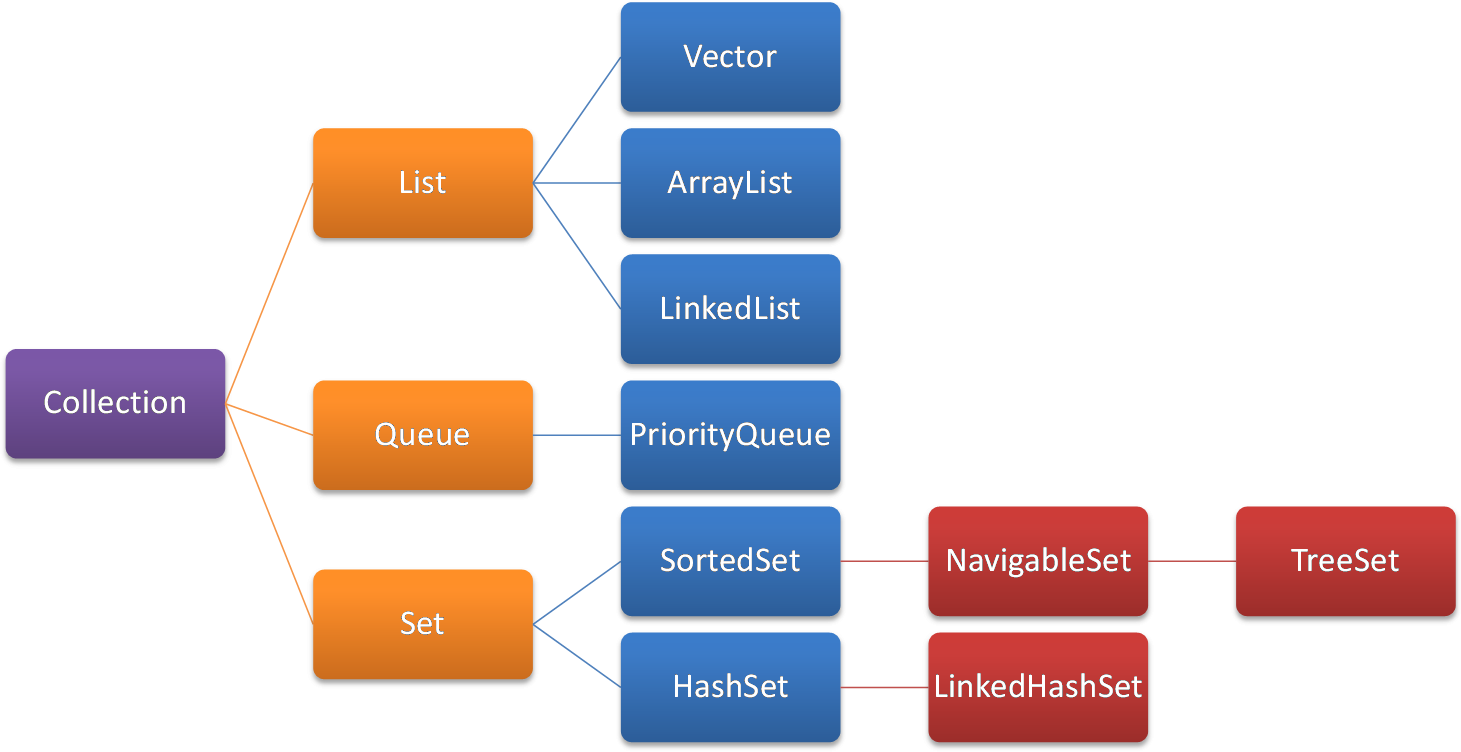
\includegraphics[width=1.0\textwidth]{set221}
  \caption[function]{Function table}
  \label{fig:function set}
\end{figure}

\section{Set and multiset} %section 2.2
\subsection{Template definition} %subsection 2.2.1
Below you can see the template definition of the \texttt{set} and \texttt{multiset} classes. 
Both classes are located in the same header file.
\begin{methodinfo}
  {<set>}
  {template < class Key, class Compare = less<Key>, class Allocator = allocator<Key> > class set;
  template < class Key, class Compare = less<Key>, class Allocator = allocator<Key> > class multiset;}
  {\texttt{Key} – the type of key stored inside the set, and therefore the type of the elements themselves

  \texttt{Compare} – the type of comparator used to perform a comparison between the \texttt{set} elements, 
  in order to ensure strict weak ordering. It can be implemented as a two-argument function, 
  or a functional object. If no comparator is provided, \texttt{less()} will be used as a default;

  \texttt{Allocator} – the type of allocator used to provide the storage allocation model.}
  {None}
  {\texttt{Set} and \texttt{multiset} are associative containers in which the elements stored 
  inside them are \texttt{keys} themselves.}
\end{methodinfo}

\subsection{Set and multiset functionality} %subsection 2.2.2
All \texttt{set} features are grouped in the table on the slide.

As you can see, there’s only one difference between these two classes, and this is why they’ll be 
described together. We’ll simply refer to both containers as \texttt{set} in the rest of this tutorial, 
with some exceptions, when their functionality differs.
\begin{figure}[htbp!]
  \centering
  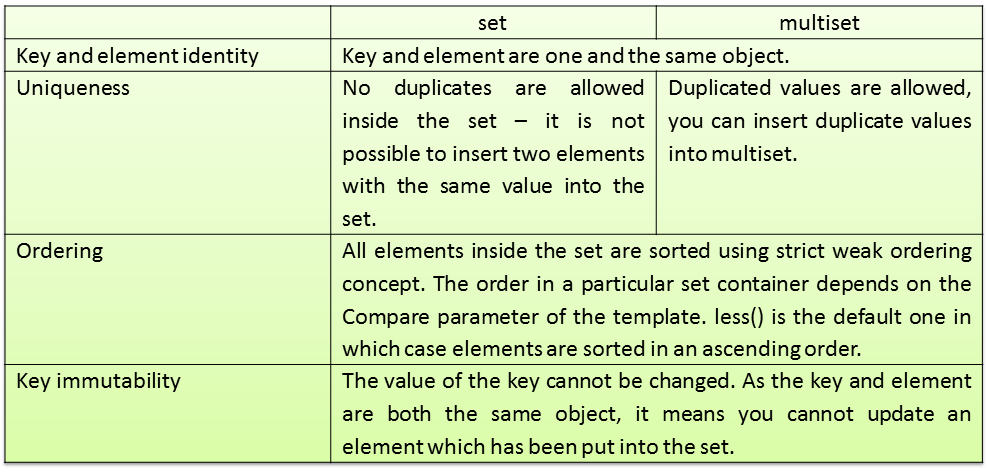
\includegraphics[width=1.0\textwidth]{set222}
  \caption[function]{Function table}
  \label{fig:function set}
\end{figure}

\subsection{Strict weak ordering \& the comparator object} %subsection 2.2.3
The elements inside the \texttt{set} are sorted using a strict weak ordering algorithm. 
In order for that to happen, two consecutive elements must be compared to one another. 
The comparison is performed using the second template parameter – \texttt{Compare}.

As you can see, the default value of that argument is \texttt{less<Key>}. In order for it to work, 
\texttt{less<Key>} requires the operator < to be defined for the type \texttt{Key}. If a particular type 
does not support this operation, a custom comparator must be created and passed during the \texttt{set} 
object definition.

Another reason to create a custom comparator is to provide some specific ordering.

A comparator \texttt{object} is required for the \texttt{set} and \texttt{multiset} to properly order the elements.

On the slide, you can see two possible prototypes of a comparator. The comparator should return \texttt{true} 
if the element k1 is placed before the element k2. Using a functional object seems to be more feasible, 
as you need to provide the comparator type as a template parameter Compare during the \texttt{set} 
object instantiation. If you intend to pass arguments to the comparator by reference, those references 
must be \texttt{const} – a key immutability restriction.

\texttt{sets} are usually preferred when you want to make sure that there’s no duplication of elements 
inside the container. The biggest issue with STL \texttt{set} implementation is that there’s no way to 
avoid ordering, which sometimes might complicate the use case; especially when we intend to put objects 
into a \texttt{set}.

You might need to provide a custom comparator, or modify a custom class by overloading the < 
(smaller than) operator, which will allow \texttt{less()} to deal with these objects.

\textcolor{green}{File name: 2.2.3.cpp} 
\lstinputlisting[language=C++]{Chapter2/codes/2.2.3.cpp} 

\subsection{Set and multiset operations} %subsection 2.2.4
\begin{itemize}
  \item constructor
  \item destructor
  \item operator=
  \item begin
  \item end
  \item rbegin
  \item rend
  \item empty
  \item size
  \item max\_size
  \item insert
  \item erase
  \item clear
  \item swap
  \item find
  \item count
  \item lower\_bound
  \item upper\_bound
  \item equal\_range
\end{itemize}

\subsection{Constructors and destructors} %subsection 2.2.5
\textbf{Name: }\\\inlinecode{C++}{constructor}\\
\textbf{Signatures: }\\
\inlinecode{C++}{explicit set ( const Compare& comp = Compare(),  const Allocator& = Allocator() );} \\
\inlinecode{C++}{template <class InputIterator>} \\
\inlinecode{C++}{set ( InputIterator first, InputIterator last, const Compare& comp = Compare(), 
const Allocator& = Allocator() );} \\
\inlinecode{C++}{set ( const set<Key,Compare,Allocator>& x );} \\
\inlinecode{C++}{explicit multiset ( const Compare& comp = Compare(), const Allocator& = Allocator() );} \\
\inlinecode{C++}{template <class InputIterator>} \\
\inlinecode{C++}{multiset ( InputIterator first, InputIterator last, const Compare& comp = Compare(), const Allocator& = Allocator() );} \\
\inlinecode{C++}{multiset ( const multiset<Key,Compare,Allocator>& x );}\\
\textbf{Parameters: }\\
\begin{itemize}
  \item \texttt{first, last} – the iterators specifying the range of elements to be inserted into 
    the container during object creation. As usual, the range includes first and excludes last;
  \item \texttt{comp} – the comparator to be used in order to provide the strict weak ordering of 
    the \texttt{set}. Its type must be the same as that specified by the template parameter Compare. 
    If this argument is omitted, the default value will be used;
  \item \texttt{unnamed allocator} – the allocator object to be used;
  \item \texttt{x} – the already existing set object; its template parameters must be set to the same values as 
    the object being created.
\end{itemize}
\textbf{Return Value: }None\\
\textbf{Description: }\\
\begin{itemize}
  \item The first constructor simply creates an empty \texttt{set} object using the optional parameters 
    \texttt{comp} and \texttt{unnamed allocator}, if they’re provided. If these arguments are not supplied, 
    this constructor becomes the default constructor.
  \item The second constructor creates a set and fills it with the elements provided by another collection. 
    The iterators \texttt{first} and \texttt{last} define the range of elements used during this initialization.
  \item The third constructor is just a copy constructor. The newly created object will be an exact copy of 
    the existing one. Both objects must be declared with the same values of the template parameters.
\end{itemize}

\begin{methodinfo}
  {destructor}
  {\~set(); \~multiset();}
  {None}
  {None}
  {It destroys the \texttt{set} container object. The destructors of all the stored objects are called, 
  and the whole allocated storage is released.}
\end{methodinfo}

\textcolor{green}{File name: 2.2.5.cpp} 
\lstinputlisting[language=C++]{Chapter2/codes/2.2.5.cpp} 

\subsection{Assignment operator} %subsection 2.2.6
\begin{methodinfo}
  {operator=}
  {set<Key,Compare,Allocator>& operator= ( const set<Key,Compare,Allocator>& x );
  multiset<Key,Compare,Allocator>& operator= ( const multiset<Key,Compare,Allocator>& x );}
  {\texttt{x} – the set object used as the source for the assignment operation;

  \texttt{Key, Compare, Allocator} – these parameters are the template parameters of 
  the \texttt{set/multiset} class.}
  {A reference to itself \texttt{(*this)}.}
  {Copies the contents of the source object to the target object. After this operation, 
  both objects are identical. The source and target objects must be defined with the same 
  values as the template parameters.}
\end{methodinfo}

\textcolor{green}{File name: 2.2.6.cpp} 
\lstinputlisting[language=C++]{Chapter2/codes/2.2.6.cpp} 

\subsection{Iterator methods} %subsection 2.2.7

\begin{methodinfo}
  {begin}
  {iterator begin (); const_iterator begin () const;}
  {None}
  {The iterator which points to the first element in the \texttt{set}}
  {This method returns an iterator which points to the first element (the key) of the \texttt{set}. 
  The function comes in two variants: const and non-const. It’s important to remember that due to the key 
  invariability of the set, there’s no functional difference between them. }
\end{methodinfo}
\begin{methodinfo}
  {end}
  {iterator end(); const_iterator end() const;}
  {None}
  {The iterator to the past-the-end element of the \texttt{set}}
  {This method returns an iterator which points to the past-the-end element (the \texttt{key}) of 
  the \texttt{set}. The past-the-end element is a virtual element located after the last element 
  of the \texttt{set}. It indicates the end of the \texttt{set}. The function comes in two variants: 
  \texttt{const} and \texttt{non-const}. It’s important to remember that due to the key invariability 
  of the \texttt{set}, there’s no functional difference between them.}
\end{methodinfo}
\begin{methodinfo}
  {rbegin}
  {reverse_iterator rbegin (); const_reverse_iterator rbegin () const;}
  {None}
  {The reverse iterator which points to the last element in the \texttt{set}(\texttt{key})}
  {This method returns a reverse iterator which points to the last element (the key) of the \texttt{set}.
  Reverse iterators iterate through the collections in reverse order – from the end to the start.
  The function comes in two variants: const and non-const. It’s important to remember that due to the key 
  invariability of the \texttt{set}, there’s no functional difference between them. }
\end{methodinfo}
\begin{methodinfo}
  {rend}
  {reverse_iterator rend(); const_reverse_iterator rend() const;}
  {None}
  {The reverse iterator of the virtual element located before the first real element of the \texttt{set}}
  {This method returns an iterator which points to the virtual element located before the first real element
  (the \texttt{key}) of the \texttt{set}. It indicates the end of the \texttt{set} in reverse order - from the 
  to the start. The function comes in two variants: \texttt{const} and \texttt{non-const}. It’s important to 
  remember that due to the key invariability of the \texttt{set}, there’s no functional difference between them.}
\end{methodinfo}

\textcolor{green}{File name: 2.2.7.cpp} 
\lstinputlisting[language=C++]{Chapter2/codes/2.2.7.cpp} 

\subsection{Size-related methods} %subsection 2.2.8

\begin{methodinfo}
  {empty}
  {bool empty () const;}
  {None}
  {This method returns \texttt{true} if the set is empty and \texttt{false} otherwise.}
  {This method is used to indicate whether the \texttt{set} is empty or not.}
\end{methodinfo}
\begin{methodinfo}
  {size}
  {size_type size() const;}
  {None}
  {The number of elements which are currently stored inside the \texttt{set}.}
  {This method returns the number of elements which are currently stored inside the \texttt{set}. 
  The size will change each time an element is added to or removed from the \texttt{set}.}
\end{methodinfo}
\begin{methodinfo}
  {max_size}
  {size_type max_size () const;}
  {None}
  {The maximum number of elements which can be held inside the \texttt{set}.}
  {This method returns the maximum physical capacity of the \texttt{set}. This value might depend on 
  the STL library implementation or operating system, and will always be constant in the same environment.}
\end{methodinfo}

\textcolor{green}{File name: 2.2.8.cpp} 
\lstinputlisting[language=C++]{Chapter2/codes/2.2.8.cpp} 

\subsection{Insert method} %subsection 2.2.9

\begin{methodinfo}
  {insert}
  {pair<iterator, bool> insert(const key_type& x );
  iterator insert (iterator position, const key_type& x );
  void insert ( iterator first, iterator last );}
  {\texttt{x}: the value to be inserted into the \texttt{set}

  \texttt{position}: the position at which value \texttt{x} should be inserted – the insertion point, 
  if chosen properly, can result in some optimization. Nonetheless, element \texttt{x} will be 
  inserted into the position which follows the existing order of the \texttt{set}.

  \texttt{first, last}: the iterators specifying the range of elements to be inserted into 
  the container during object creation. As usual, the range includes \texttt{first} and excludes \texttt{last}.}
  {The first version (\texttt{set}) returns a structure \texttt{pair} in which the \texttt{first} field is 
  an iterator of the newly inserted element, or an already existing element in the \texttt{set}. 
  The information stating which scenario has happened is stored inside the second field: \texttt{true} – 
  insertion, \texttt{false} – a value already exists.

  the second version (\texttt{set}) returns an iterator which points either to the newly inserted element, 
  or to an already existing element.

  for \texttt{multiset}, the returned value always points to the newly inserted element.}
  {The function \texttt{insert()} is used to put new values into a \texttt{set}. 
  Each successful call of this method will effectively increase the size of the \texttt{set}. 
  As the \texttt{set} container does not allow duplicate values, each element to be inserted is 
  checked to make sure that it doesn’t violate this condition. If it does, the insertion will be unsuccessful.

  As \texttt{multiset} allows for duplicate elements, there can never be an unsuccessful scenario for 
  a call to \texttt{insert()}.

  Another restriction is related to the order of the elements in the \texttt{set}. 
  The new element will be placed at a position which follows the set-ordering policy. 
  As we stated earlier, the parameter \texttt{position} in the second version of this method 
  has only an informative meaning, suggesting a possible insertion point, but can result in 
  performance improvements during the insertion process. A newly inserted element is obtained by 
  creating a copy of parameter \texttt{x}.
  
  The last version of \texttt{insert()} inserts elements from range defined by the iterators 
  \texttt{first} and \texttt{last}. All these restrictions still apply for both classes respectively.}
\end{methodinfo}

\textcolor{green}{File name: 2.2.9.cpp} 
\lstinputlisting[language=C++]{Chapter2/codes/2.2.9.cpp} 

\subsection{Erase methods} %section 2.2.10
Erase methods: removing elements from the container.
\begin{methodinfo}
  {erase}
  {void erase ( iterator position );
  size_type erase ( const key_type& x );
  void erase ( iterator first, iterator last );}
  {\texttt{position}: the iterator pointing to the element to be removed. 

  \texttt{x}: the element (\texttt{key}) to be removed from the \texttt{set}, \inlinecode{C++}{key_type} 
  is an alias to \texttt{Key}, which is the \texttt{first} template parameter.

  \texttt{first, last}: the iterators specifying the range of elements to be removed from the \texttt{set}. 
  As usual, the range includes first and excludes last.}
  {The number of elements removed: for the \texttt{set}, it is either 1 if value \texttt{x} has been removed, 
  or 0 otherwise; for a \texttt{multiset}, the function returns the number of times value \texttt{x} is 
  presented in the \texttt{multiset}, or 0 if it isn’t found at all.}
  {This function removes elements from the collection. As a result, the \texttt{set} size will be decreased 
  and the destructor of each deleted element will be called. The deletion might be performed using one of 
  three possible methods:
  
  iterator
  
  key value
  
  range of iterators}
\end{methodinfo}

\textcolor{green}{File name: 2.2.10.cpp} 
\lstinputlisting[language=C++]{Chapter2/codes/2.2.10.cpp} 

\subsection{swap method} %subsection 2.2.11
\begin{methodinfo}
  {swap}
  {void swap ( set<Key,Compare,Allocator>& st );}
  {\texttt{st}: the other set container identical in meaning to the template parameters with this method’s caller.}
  {None}
  {This function performs the exchange of all contents between two set containers. After the call, all the elements stored in the set will be placed in st and vice versa. All iterators, references and pointers obtained before the call are still valid, but in relation to the swapped set objects. No construction or destruction of elements inside either of the sets is performed during the call.}
\end{methodinfo}

\textcolor{green}{File name: 2.2.11.cpp} 
\lstinputlisting[language=C++]{Chapter2/codes/2.2.11.cpp} 

\subsection{find method} %subsection 2.2.12
\begin{methodinfo}
  {find}
  {iterator find ( const key_type& x ) const;}
  {\texttt{x}: the value to be searched for in the set.}
  {If successful, an iterator to the found element is returned. If the value cannot be found, 
  the function returns \texttt{set::end()} (past-the-end element)}
  {The function \texttt{find()} looks for value x inside the set. If the value is found, the iterator to 
  it is returned. A search failure is indicated by returning the \texttt{set::end()} value.
  
  For a \texttt{multiset}, this function returns an iterator pointing to the first place in which this value is 
  present inside the container.}
\end{methodinfo}

\textcolor{green}{File name: 2.2.12.cpp} 
\lstinputlisting[language=C++]{Chapter2/codes/2.2.12.cpp} 

\subsection{Count method} %subsection 2.2.13
\begin{methodinfo}
  {count}
  {size_type count ( const key_type& x ) const;}
  {\texttt{x}: the value to be looked for in the set.}
  {Returns the number of times value \texttt{x} has been found in the \texttt{set/multiset}. In the case of 
  a \texttt{set}, it either returns 1 if the searched value has been found, or 0 otherwise.}
  {The function \texttt{count()} looks for value \texttt{x} and returns the number of times this value 
  occurs in the \texttt{set/multiset}. Since the set does not allow for duplicates, this means that 
  the function returns either 1 or 0.

  For a \texttt{multiset}, the returned number can, of course, be greater than 1.}
\end{methodinfo}

\textcolor{green}{File name: 2.2.13.cpp} 
\lstinputlisting[language=C++]{Chapter2/codes/2.2.13.cpp} 

\subsection{Bounds related methods} %subsection 2.2.13
\begin{methodinfo}
  {lower_bound}
  {iterator lower_bound ( const key_type& x ) const;}
  {\texttt{x}: the value to be looked for inside the set.}
  {The iterator to the first element which is greater than or equal to the value \texttt{x}.}
  {This method searches the \texttt{set} for the first value which is greater than or equal to 
  the given parameter \texttt{x} (it does not compare less than). Because sets are ordered containers, 
  it means that all elements between the returned iterator and \texttt{set::end} will be greater than or 
  equal to the searched value.}
\end{methodinfo}
\begin{methodinfo}
  {upper_bound}
  {iterator upper_bound ( const key_type& x ) const;}
  {\texttt{x}: the value to be looked for.}
  {The iterator to the first element which is greater than value \texttt{x}.}
  {This method searches the \texttt{set} for the first value which is greater than (strict comparison) 
  the given parameter \texttt{x}. Because sets are ordered containers, it means that all elements between 
  the returned iterator and the \texttt{set::end} will be greater than the searched value.}
\end{methodinfo}
\begin{methodinfo}
  {equal_range}
  {pair<iterator,iterator> equal_range ( const key_type& x ) const;}
  {\texttt{x}: the value to be searched for in the \texttt{set/multiset.}}
  {A pair of iterators whose values depend on the result of the search:

  if the search is successful, the first iterator points to the first element which is not less than 
  (greater than or equal to) the requested value \texttt{x}, whereas the second iterator points to 
  the first element greater than the given value \texttt{x}

  if an element that is not less than \texttt{x} cannot be found, then both returned iterators point to the 
  first element greater than \texttt{x}, or, if there is no greater element, to the past-the-end element

  if an element that is not less than \texttt{x} is found, but an element greater than \texttt{x} is not, 
  then the first returned iterator points to the found element, whereas the second iterator points to 
  the past-the-end element.}
  {The method \inlinecode{C++}{equal_range()} searches the \texttt{set} for the first element which is 
  greater than or equal to value \texttt{x}, and the first element which is greater than value \texttt{x}.

  Since the \texttt{set} is an ordered container, in the event of it being successful, the search produces 
  a \texttt{range} of elements, containing exactly one element.

  For a \texttt{multiset} container, the returned range can have more than one element. This function is 
  just a combination of the \inlinecode{C++}{lower_bound()} and \inlinecode{C++}{upper_bound()} functions.


  The first field of the returned pair of iterators should point to the element greater than or 
  equal to \texttt{x} (\inlinecode{C++}{lower_bound()}), whereas the second field should point to 
  an element greater than \texttt{x} (\inlinecode{C++}{upper_bound()}).}
\end{methodinfo}

\textcolor{green}{File name: 2.2.14.cpp} 
\lstinputlisting[language=C++]{Chapter2/codes/2.2.14.cpp} 

\section{Map and multimap} %section 2.3
\subsection{Introduction to map containers} %subsection 2.3.1

























%*************************comment**********************************************
\begin{comment}
  \ifpdf
      \graphicspath{{Chapter2/Figs/Raster/}{Chapter2/Figs/PDF/}{Chapter2/Figs/}}
  \else
      \graphicspath{{Chapter2/Figs/Vector/}{Chapter2/Figs/}}
  \fi
  
  \section[Short title]{Reasonably long section title}
  
  % Uncomment this line, when you have siunitx package loaded.
  %The SI Units for dynamic viscosity is \si{\newton\second\per\metre\squared}.
  I'm going to randomly include a picture Figure~\ref{fig:minion}.
  
  
  If you have trouble viewing this document contact Krishna at: \href{mailto:kks32@cam.ac.uk}{kks32@cam.ac.uk} or raise an issue at \url{https://github.com/kks32/phd-thesis-template/}
  
  
  \begin{figure}[htbp!] 
  \centering    
  
\includegraphics[width=1.0\textwidth]{minion}
  \caption[Minion]{This is just a long figure caption for the minion in Despicable Me from Pixar}
  \label{fig:minion}
  \end{figure}
  
  
  \section*{Enumeration}
  Lorem ipsum dolor sit amet, consectetur adipiscing elit. Sed vitae laoreet lectus. Donec lacus quam, malesuada ut erat vel, consectetur eleifend tellus. Aliquam non feugiat lacus. Interdum et malesuada fames ac ante ipsum primis in faucibus. Quisque a dolor sit amet dui malesuada malesuada id ac metus. Phasellus posuere egestas mauris, sed porta arcu vulputate ut. Donec arcu erat, ultrices et nisl ut, ultricies facilisis urna. Quisque iaculis, lorem non maximus pretium, dui eros auctor quam, sed sodales libero felis vel orci. Aliquam neque nunc, elementum id accumsan eu, varius eu enim. Aliquam blandit ante et ligula tempor pharetra. Donec molestie porttitor commodo. Integer rutrum turpis ac erat tristique cursus. Sed venenatis urna vel tempus venenatis. Nam eu rhoncus eros, et condimentum elit. Quisque risus turpis, aliquam eget euismod id, gravida in odio. Nunc elementum nibh risus, ut faucibus mauris molestie eu.
   Vivamus quis nunc nec nisl vulputate fringilla. Duis tempus libero ac justo laoreet tincidunt. Fusce sagittis gravida magna, pharetra venenatis mauris semper at. Nullam eleifend felis a elementum sagittis. In vel turpis eu metus euismod tempus eget sit amet tortor. Donec eu rhoncus libero, quis iaculis lectus. Aliquam erat volutpat. Proin id ullamcorper tortor. Fusce vestibulum a enim non volutpat. Nam ut interdum nulla. Proin lacinia felis malesuada arcu aliquet fringilla. Aliquam condimentum, tellus eget maximus porttitor, quam sem luctus massa, eu fermentum arcu diam ac massa. Praesent ut quam id leo molestie rhoncus. Praesent nec odio eget turpis bibendum eleifend non sit amet mi. Curabitur placerat finibus velit, eu ultricies risus imperdiet ut. Suspendisse lorem orci, luctus porta eros a, commodo maximus nisi.
  
  Nunc et dolor diam. Phasellus eu justo vitae diam vehicula tristique. Vestibulum vulputate cursus turpis nec commodo. Etiam elementum sit amet erat et pellentesque. In eu augue sed tortor mollis tincidunt. Mauris eros dui, sagittis vestibulum vestibulum vitae, molestie a velit. Donec non felis ut velit aliquam convallis sit amet sit amet velit. Aliquam vulputate, elit in lacinia lacinia, odio lacus consectetur quam, sit amet facilisis mi justo id magna. Curabitur aliquet pulvinar eros. Cras metus enim, tristique ut magna a, interdum egestas nibh. Aenean lorem odio, varius a sollicitudin non, cursus a odio. Vestibulum ante ipsum primis in faucibus orci luctus et ultrices posuere cubilia Curae; 
  \begin{enumerate}
  \item The first topic is dull
  \item The second topic is duller
  \begin{enumerate}
  \item The first subtopic is silly
  \item The second subtopic is stupid
  \end{enumerate}
  \item The third topic is the dullest
  \end{enumerate}
  Morbi bibendum est aliquam, hendrerit dolor ac, pretium sem. Nunc molestie, dui in euismod finibus, nunc enim viverra enim, eu mattis mi metus id libero. Cras sed accumsan justo, ut volutpat ipsum. Nam faucibus auctor molestie. Morbi sit amet eros a justo pretium aliquet. Maecenas tempor risus sit amet tincidunt tincidunt. Curabitur dapibus gravida gravida. Vivamus porta ullamcorper nisi eu molestie. Ut pretium nisl eu facilisis tempor. Nulla rutrum tincidunt justo, id placerat lacus laoreet et. Sed cursus lobortis vehicula. Donec sed tortor et est cursus pellentesque sit amet sed velit. Proin efficitur posuere felis, porta auctor nunc. Etiam non porta risus. Pellentesque lacinia eros at ante iaculis, sed aliquet ipsum volutpat. Suspendisse potenti.
  
  Ut ultrices lectus sed sagittis varius. Nulla facilisi. Nullam tortor sem, placerat nec condimentum eu, tristique eget ex. Nullam pretium tellus ut nibh accumsan elementum. Aliquam posuere gravida tellus, id imperdiet nulla rutrum imperdiet. Nulla pretium ullamcorper quam, non iaculis orci consectetur eget. Curabitur non laoreet nisl. Maecenas lacinia, lorem vel tincidunt cursus, odio lorem aliquet est, gravida auctor arcu urna id enim. Morbi accumsan bibendum ipsum, ut maximus dui placerat vitae. Nullam pretium ac tortor nec venenatis. Nunc non aliquet neque. 
  
  \section*{Itemize}
  \begin{itemize}
  \item The first topic is dull
  \item The second topic is duller
  \begin{itemize}
  \item The first subtopic is silly
  \item The second subtopic is stupid
  \end{itemize}
  \item The third topic is the dullest
  \end{itemize}
  
  \section*{Description}
  \begin{description}
  \item[The first topic] is dull
  \item[The second topic] is duller
  \begin{description}
  \item[The first subtopic] is silly
  \item[The second subtopic] is stupid
  \end{description}
  \item[The third topic] is the dullest
  \end{description}
  
  
  \clearpage
  
  \tochide\section{Hidden section}
  \textbf{Lorem ipsum dolor sit amet}, \textit{consectetur adipiscing elit}. In magna nisi, aliquam id blandit id, congue ac est. Fusce porta consequat leo. Proin feugiat at felis vel consectetur. Ut tempus ipsum sit amet congue posuere. Nulla varius rutrum quam. Donec sed purus luctus, faucibus velit id, ultrices sapien. Cras diam purus, tincidunt eget tristique ut, egestas quis nulla. Curabitur vel iaculis lectus. Nunc nulla urna, ultrices et eleifend in, accumsan ut erat. In ut ante leo. Aenean a lacinia nisl, sit amet ullamcorper dolor. Maecenas blandit, tortor ut scelerisque congue, velit diam volutpat metus, sed vestibulum eros justo ut nulla. Etiam nec ipsum non enim luctus porta in in massa. Cras arcu urna, malesuada ut tellus ut, pellentesque mollis risus.Morbi vel tortor imperdiet arcu auctor mattis sit amet eu nisi. Nulla gravida urna vel nisl egestas varius. Aliquam posuere ante quis malesuada dignissim. Mauris ultrices tristique eros, a dignissim nisl iaculis nec. Praesent dapibus tincidunt mauris nec tempor. Curabitur et consequat nisi. Quisque viverra egestas risus, ut sodales enim blandit at. Mauris quis odio nulla. Cras euismod turpis magna, in facilisis diam congue non. Mauris faucibus nisl a orci dictum, et tempus mi cursus.
  
  Etiam elementum tristique lacus, sit amet eleifend nibh eleifend sed \footnote{My footnote goes blah blah blah! \dots}. Maecenas dapibu augue ut urna malesuada, non tempor nibh mollis. Donec sed sem sollicitudin, convallis velit aliquam, tincidunt diam. In eu venenatis lorem. Aliquam non augue porttitor tellus faucibus porta et nec ante. Proin sodales, libero vitae commodo sodales, dolor nisi cursus magna, non tincidunt ipsum nibh eget purus. Nam rutrum tincidunt arcu, tincidunt vulputate mi sagittis id. Proin et nisi nec orci tincidunt auctor et porta elit. Praesent eu dolor ac magna cursus euismod. Integer non dictum nunc.
  
  
  \begin{landscape}
  
  \section*{Subplots}
  I can cite Wall-E (see Fig.~\ref{fig:WallE}) and Minions in despicable me (Fig.~\ref{fig:Minnion}) or I can cite the whole figure as Fig.~\ref{fig:animations}
  
  
  \begin{figure}
    \centering
    \begin{subfigure}[b]{0.3\textwidth}
      
\includegraphics[width=\textwidth]{TomandJerry}
      \caption{Tom and Jerry}
      \label{fig:TomJerry}   
    \end{subfigure}             
    \begin{subfigure}[b]{0.3\textwidth}
      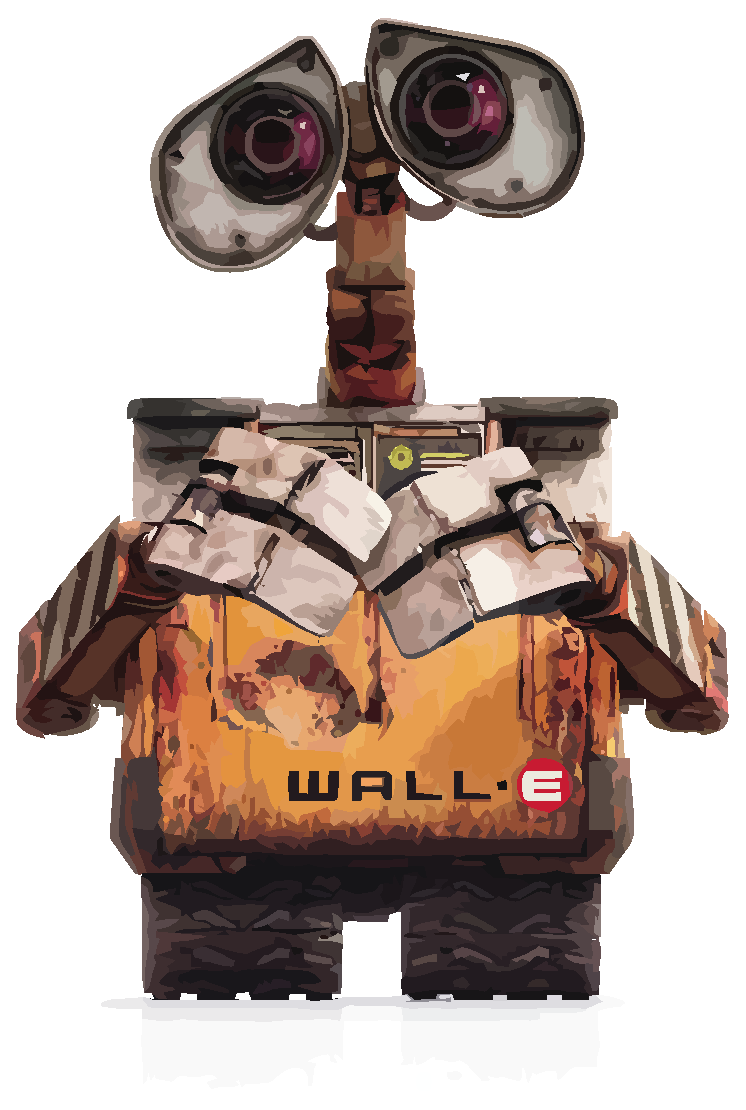
\includegraphics[width=\textwidth]{WallE}
      \caption{Wall-E}
      \label{fig:WallE}
    \end{subfigure}             
    \begin{subfigure}[b]{0.3\textwidth}
      
\includegraphics[width=\textwidth]{minion}
      \caption{Minions}
      \label{fig:Minnion}
    \end{subfigure}
    \caption{Best Animations}
    \label{fig:animations}
  \end{figure}
  
  
  \end{landscape}

\end{comment}


% ********************************** Back Matter *******************************
% Backmatter should be commented out, if you are using appendices after References
%\backmatter

% ********************************** Bibliography ******************************
\begin{spacing}{0.9}

% To use the conventional natbib style referencing
% Bibliography style previews: http://nodonn.tipido.net/bibstyle.php
% Reference styles: http://sites.stat.psu.edu/~surajit/present/bib.htm

\bibliographystyle{apalike}
%\bibliographystyle{unsrt} % Use for unsorted references  
%\bibliographystyle{plainnat} % use this to have URLs listed in References
\cleardoublepage
\bibliography{References/references} % Path to your References.bib file


% If you would like to use BibLaTeX for your references, pass `custombib' as
% an option in the document class. The location of 'reference.bib' should be
% specified in the preamble.tex file in the custombib section.
% Comment out the lines related to natbib above and uncomment the following line.

%\printbibliography[heading=bibintoc, title={References}]


\end{spacing}

% ********************************** Appendices ********************************

\begin{appendices} % Using appendices environment for more functunality

%!TEX root = ../thesis.tex
% ******************************* Thesis Appendix A ****************************
\chapter{How to install \LaTeX} 

\section*{Windows OS}

\subsection*{TeXLive package - full version}
\begin{enumerate}
\item	Download the TeXLive ISO (2.2GB) from\\
\href{https://www.tug.org/texlive/}{https://www.tug.org/texlive/}
\item	Download WinCDEmu (if you don't have a virtual drive) from \\
\href{http://wincdemu.sysprogs.org/download/}
{http://wincdemu.sysprogs.org/download/}
\item	To install Windows CD Emulator follow the instructions at\\
\href{http://wincdemu.sysprogs.org/tutorials/install/}
{http://wincdemu.sysprogs.org/tutorials/install/}
\item	Right click the iso and mount it using the WinCDEmu as shown in \\
\href{http://wincdemu.sysprogs.org/tutorials/mount/}{
http://wincdemu.sysprogs.org/tutorials/mount/}
\item	Open your virtual drive and run setup.pl
\end{enumerate}

or

\subsection*{Basic MikTeX - \TeX~ distribution}
\begin{enumerate}
\item	Download Basic-MiK\TeX (32bit or 64bit) from\\
\href{http://miktex.org/download}{http://miktex.org/download}
\item	Run the installer 
\item	To add a new package go to Start >> All Programs >> MikTex >> Maintenance (Admin) and choose Package Manager
\item	Select or search for packages to install
\end{enumerate}

\subsection*{TexStudio - \TeX~ editor}
\begin{enumerate}
\item	Download TexStudio from\\
\href{http://texstudio.sourceforge.net/\#downloads}
{http://texstudio.sourceforge.net/\#downloads} 
\item	Run the installer
\end{enumerate}

\section*{Mac OS X}
\subsection*{MacTeX - \TeX~ distribution}
\begin{enumerate}
\item	Download the file from\\
\href{https://www.tug.org/mactex/}{https://www.tug.org/mactex/}
\item	Extract and double click to run the installer. It does the entire configuration, sit back and relax.
\end{enumerate}

\subsection*{TexStudio - \TeX~ editor}
\begin{enumerate}
\item	Download TexStudio from\\
\href{http://texstudio.sourceforge.net/\#downloads}
{http://texstudio.sourceforge.net/\#downloads} 
\item	Extract and Start
\end{enumerate}


\section*{Unix/Linux}
\subsection*{TeXLive - \TeX~ distribution}
\subsubsection*{Getting the distribution:}
\begin{enumerate}
\item	TexLive can be downloaded from\\
\href{http://www.tug.org/texlive/acquire-netinstall.html}
{http://www.tug.org/texlive/acquire-netinstall.html}.
\item	TexLive is provided by most operating system you can use (rpm,apt-get or yum) to get TexLive distributions
\end{enumerate}

\subsubsection*{Installation}
\begin{enumerate}
\item	Mount the ISO file in the mnt directory
\begin{verbatim}
mount -t iso9660 -o ro,loop,noauto /your/texlive####.iso /mnt
\end{verbatim}

\item	Install wget on your OS (use rpm, apt-get or yum install)
\item	Run the installer script install-tl.
\begin{verbatim}
	cd /your/download/directory
	./install-tl
\end{verbatim}
\item	Enter command `i' for installation

\item	Post-Installation configuration:\\
\href{http://www.tug.org/texlive/doc/texlive-en/texlive-en.html\#x1-320003.4.1}
{http://www.tug.org/texlive/doc/texlive-en/texlive-en.html\#x1-320003.4.1} 
\item	Set the path for the directory of TexLive binaries in your .bashrc file
\end{enumerate}

\subsubsection*{For 32bit OS}
For Bourne-compatible shells such as bash, and using Intel x86 GNU/Linux and a default directory setup as an example, the file to edit might be \begin{verbatim}
edit $~/.bashrc file and add following lines
PATH=/usr/local/texlive/2011/bin/i386-linux:$PATH; 
export PATH 
MANPATH=/usr/local/texlive/2011/texmf/doc/man:$MANPATH;
export MANPATH 
INFOPATH=/usr/local/texlive/2011/texmf/doc/info:$INFOPATH;
export INFOPATH
\end{verbatim}
\subsubsection*{For 64bit OS}
\begin{verbatim}
edit $~/.bashrc file and add following lines
PATH=/usr/local/texlive/2011/bin/x86_64-linux:$PATH;
export PATH 
MANPATH=/usr/local/texlive/2011/texmf/doc/man:$MANPATH;
export MANPATH 
INFOPATH=/usr/local/texlive/2011/texmf/doc/info:$INFOPATH;
export INFOPATH

\end{verbatim}



%\subsection{Installing directly using Linux packages} 
\subsubsection*{Fedora/RedHat/CentOS:}
\begin{verbatim} 
sudo yum install texlive 
sudo yum install psutils 
\end{verbatim}


\subsubsection*{SUSE:}
\begin{verbatim}
sudo zypper install texlive
\end{verbatim}


\subsubsection*{Debian/Ubuntu:}
\begin{verbatim} 
sudo apt-get install texlive texlive-latex-extra 
sudo apt-get install psutils
\end{verbatim}

%!TEX root = ../thesis.tex
% ******************************* Thesis Appendix B ********************************

\chapter{Installing the CUED class file}

\LaTeX.cls files can be accessed system-wide when they are placed in the
<texmf>/tex/latex directory, where <texmf> is the root directory of the user’s \TeX installation. On systems that have a local texmf tree (<texmflocal>), which
may be named ``texmf-local'' or ``localtexmf'', it may be advisable to install packages in <texmflocal>, rather than <texmf> as the contents of the former, unlike that of the latter, are preserved after the \LaTeX system is reinstalled and/or upgraded.

It is recommended that the user create a subdirectory <texmf>/tex/latex/CUED for all CUED related \LaTeX class and package files. On some \LaTeX systems, the directory look-up tables will need to be refreshed after making additions or deletions to the system files. For \TeX Live systems this is accomplished via executing ``texhash'' as root. MIK\TeX users can run ``initexmf -u'' to accomplish the same thing.

Users not willing or able to install the files system-wide can install them in their personal directories, but will then have to provide the path (full or relative) in addition to the filename when referring to them in \LaTeX.



\end{appendices}

% *************************************** Index ********************************
\printthesisindex % If index is present

\end{document}
